\documentclass[a4wide, 10pt]{article}
\usepackage{a4, fullpage}
\usepackage[section]{placeins}
\usepackage{float}
\setlength{\parskip}{0.15cm}
\setlength{\parindent}{0cm}
\usepackage{graphicx}
\usepackage{caption}
\usepackage{subcaption}
\usepackage{amssymb}
\usepackage{amsmath}
\usepackage{hyperref}
\usepackage{graphicx,wrapfig,lipsum}
\begin{document}

\title{Maps, Sets and Fractals}

\author{William Springsteen \and Kiran Patel \and Stefan Klas \and Rory Fayed}

\maketitle

\section{Introduction}

The world of non-linear dynamics of discrete maps truly is a fascinating one. The
 definition of the word \emph{chaos} in the dictionary is \emph{'Complete disorder
  and confusion'}\cite{Chaos in Dictionary}. The same source also defines chaos, 
   this time in a purely scientific context, as \emph{'The property of a complex 
    system whose behaviour is so unpredictable as to appear random, owing to great 
     sensitivity to small changes in conditions'}. From this, you would assume that
      chaos, which will be investigated in this report, is true randomness, or something
       extremely close to that. It turns out that there is, in fact, order arising in 
        chaotic systems. This is an example of how most things in non-linear dynamics of
         discrete maps are not as they first seem - Things that seem like they
          would have an obvious result, or no result at all, may end up having
           extraordinary results.

In this report, some one-dimensional discrete maps will be investigated and compared - the Verhulst map, the logistic map, and the trigonometric map. The Mandelbrot set, a one-dimensional complex map which is a specific 
    implementation of the Verhulst process, will then be  investigated, along with 
     Julia sets, which occur inside the Mandelbrot set, and Boll's results.

\section{One Dimensional Discrete Non-Linear Maps}

In this section, some one dimensional discrete non-linear maps will be investigated
 and compared. The Verhulst map, the logistic map, and the trigonometric map are the three maps to be investigated.

\subsection{Verhulst Map}

The Verhulst map, named after Pierre François Verhulst, is a one-dimensional
 discrete map designed to model bounded population growth. In 1832, Verhulst and his
  old maths professor, and good friend, Adolphe Quetelet, started working on
   modelling population growth\cite{Pierre Verhulst Biography}. This began when Quetelet
    was asked to draw up mortality tables for the newly independent Belgium, and Quetelet
     asked Verhulst to help in doing this. Prior to Verhulst and Quetelet working on
      modelling population growth, it was believed that an increasing population followed a
       geometric sequence. Quetelet and Verhulst both thought this was wrong, but
        both had differing ideas. Quetelet proposed that a geometric progression
         model of population growth would be wrong over a long period of time due to
          limiting factors, forming a kind of resistance to the growth, such as size
           of the country, and the amount of food available. In 1835, Quetelet
            suggested that these limiting factors were proportional to the square of
             the speed of population growth, as is the case in mechanics\cite{Information 
              on Veruhlst and Verhulst/Logistic Maps}.
               Verhulst took inspiration from this, but in 1838, he published a paper, 
                \emph{Notice sur la loi que la population suit dans son accroissement}, 
                 that claimed it would be better to model this with a differential
                  equation\cite{Pierre Verhulst Biography}. This differential equation
                   became known as the Verhulst map, defined by: 

\[
  x_{k+1} = x_{k} + rx_{k}(1 - x_{k}) \textrm{, for \emph{k}} \geq 0
\]

Our initial approach to investigate this process was to depict the process iteratively 
 using a cobweb diagram. This was done in Matlab by plotting $x_{k+1}$ against
  $x_{k}$ for a number of iterations (1000) that was large enough to show any points where 
   the value of the function was tending to, the name of these points are called attractors.
    Moving between the range $ 0 \leq r < 2 $, you are able to see that there are specific
     values of r where the process changes from having $n$ attractors, say, to having $2n$
      attractors. At these $r$ values where the number of attractors doubles it is known as
       period doubling with period size $n$: 

%First 5 images       
\begin{figure}[H]
        \centering
        \begin{subfigure}[b]{0.19\textwidth}
                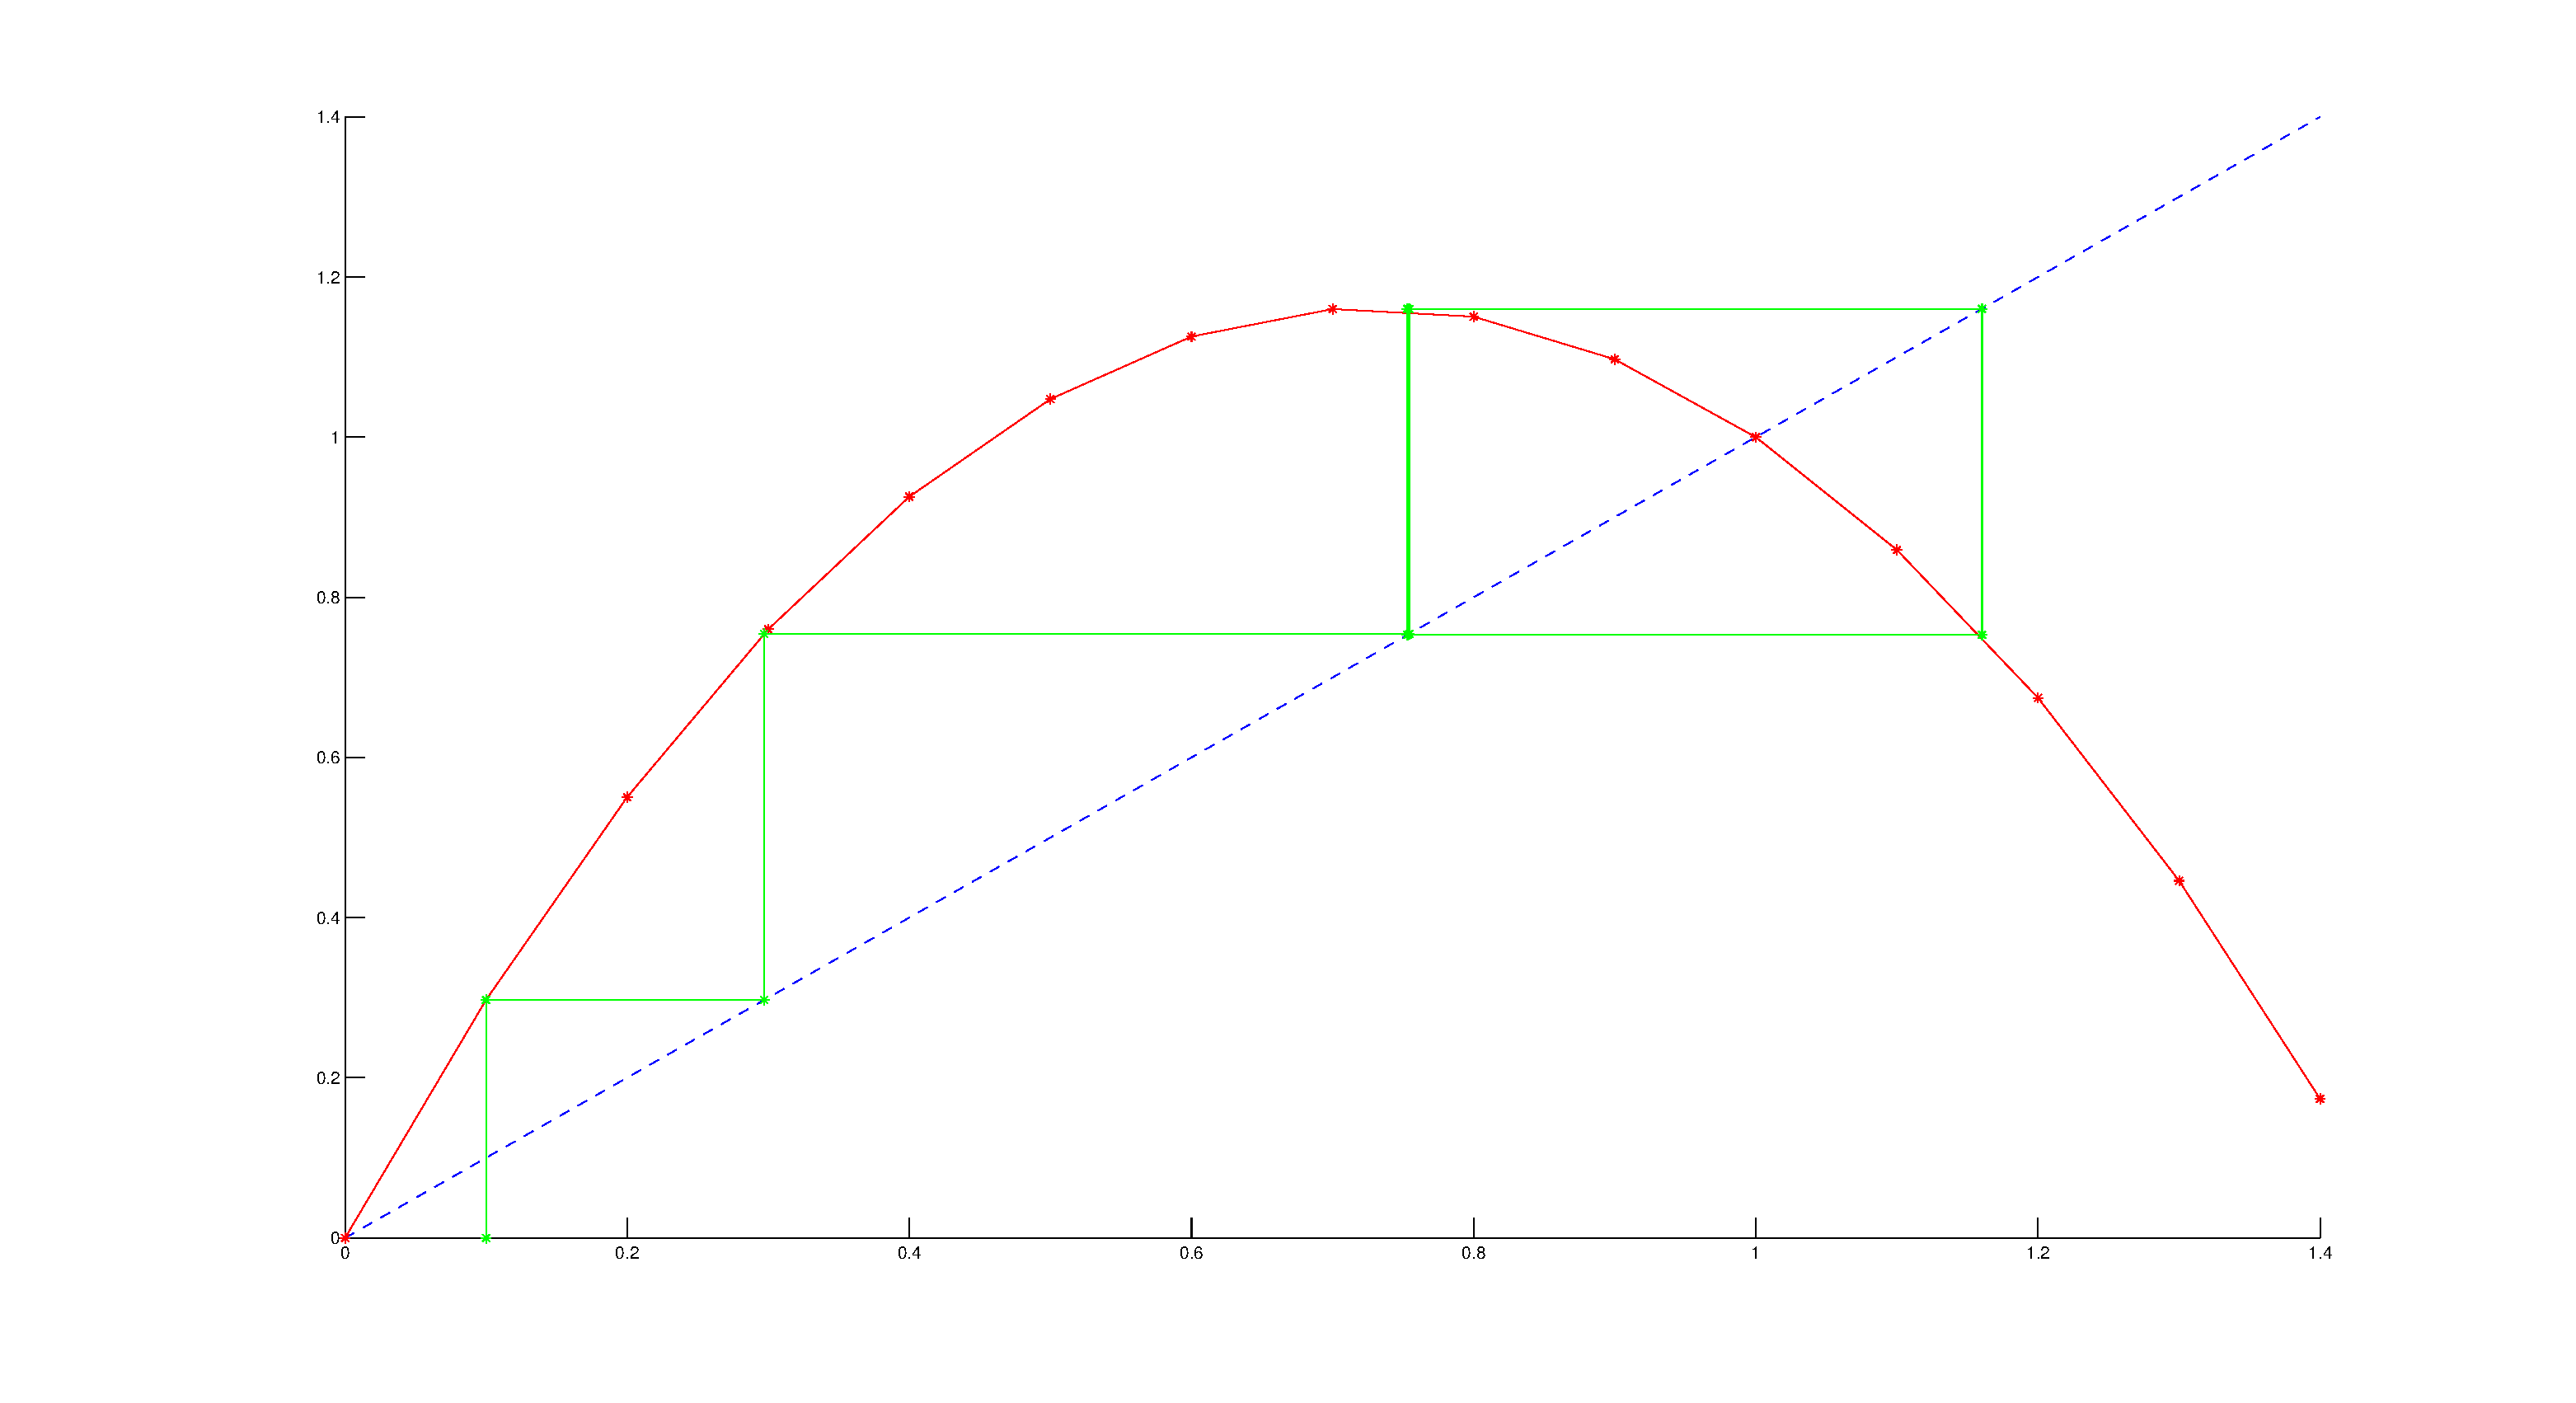
\includegraphics[width=\textwidth]{EPSFiles/CobwebPD_2_VMap}
                \caption{4 Attractors, \newline \hspace{2cm} r = 2.19}
                \label{fig:Cobweb2}
        \end{subfigure}
        \begin{subfigure}[b]{0.19\textwidth}
                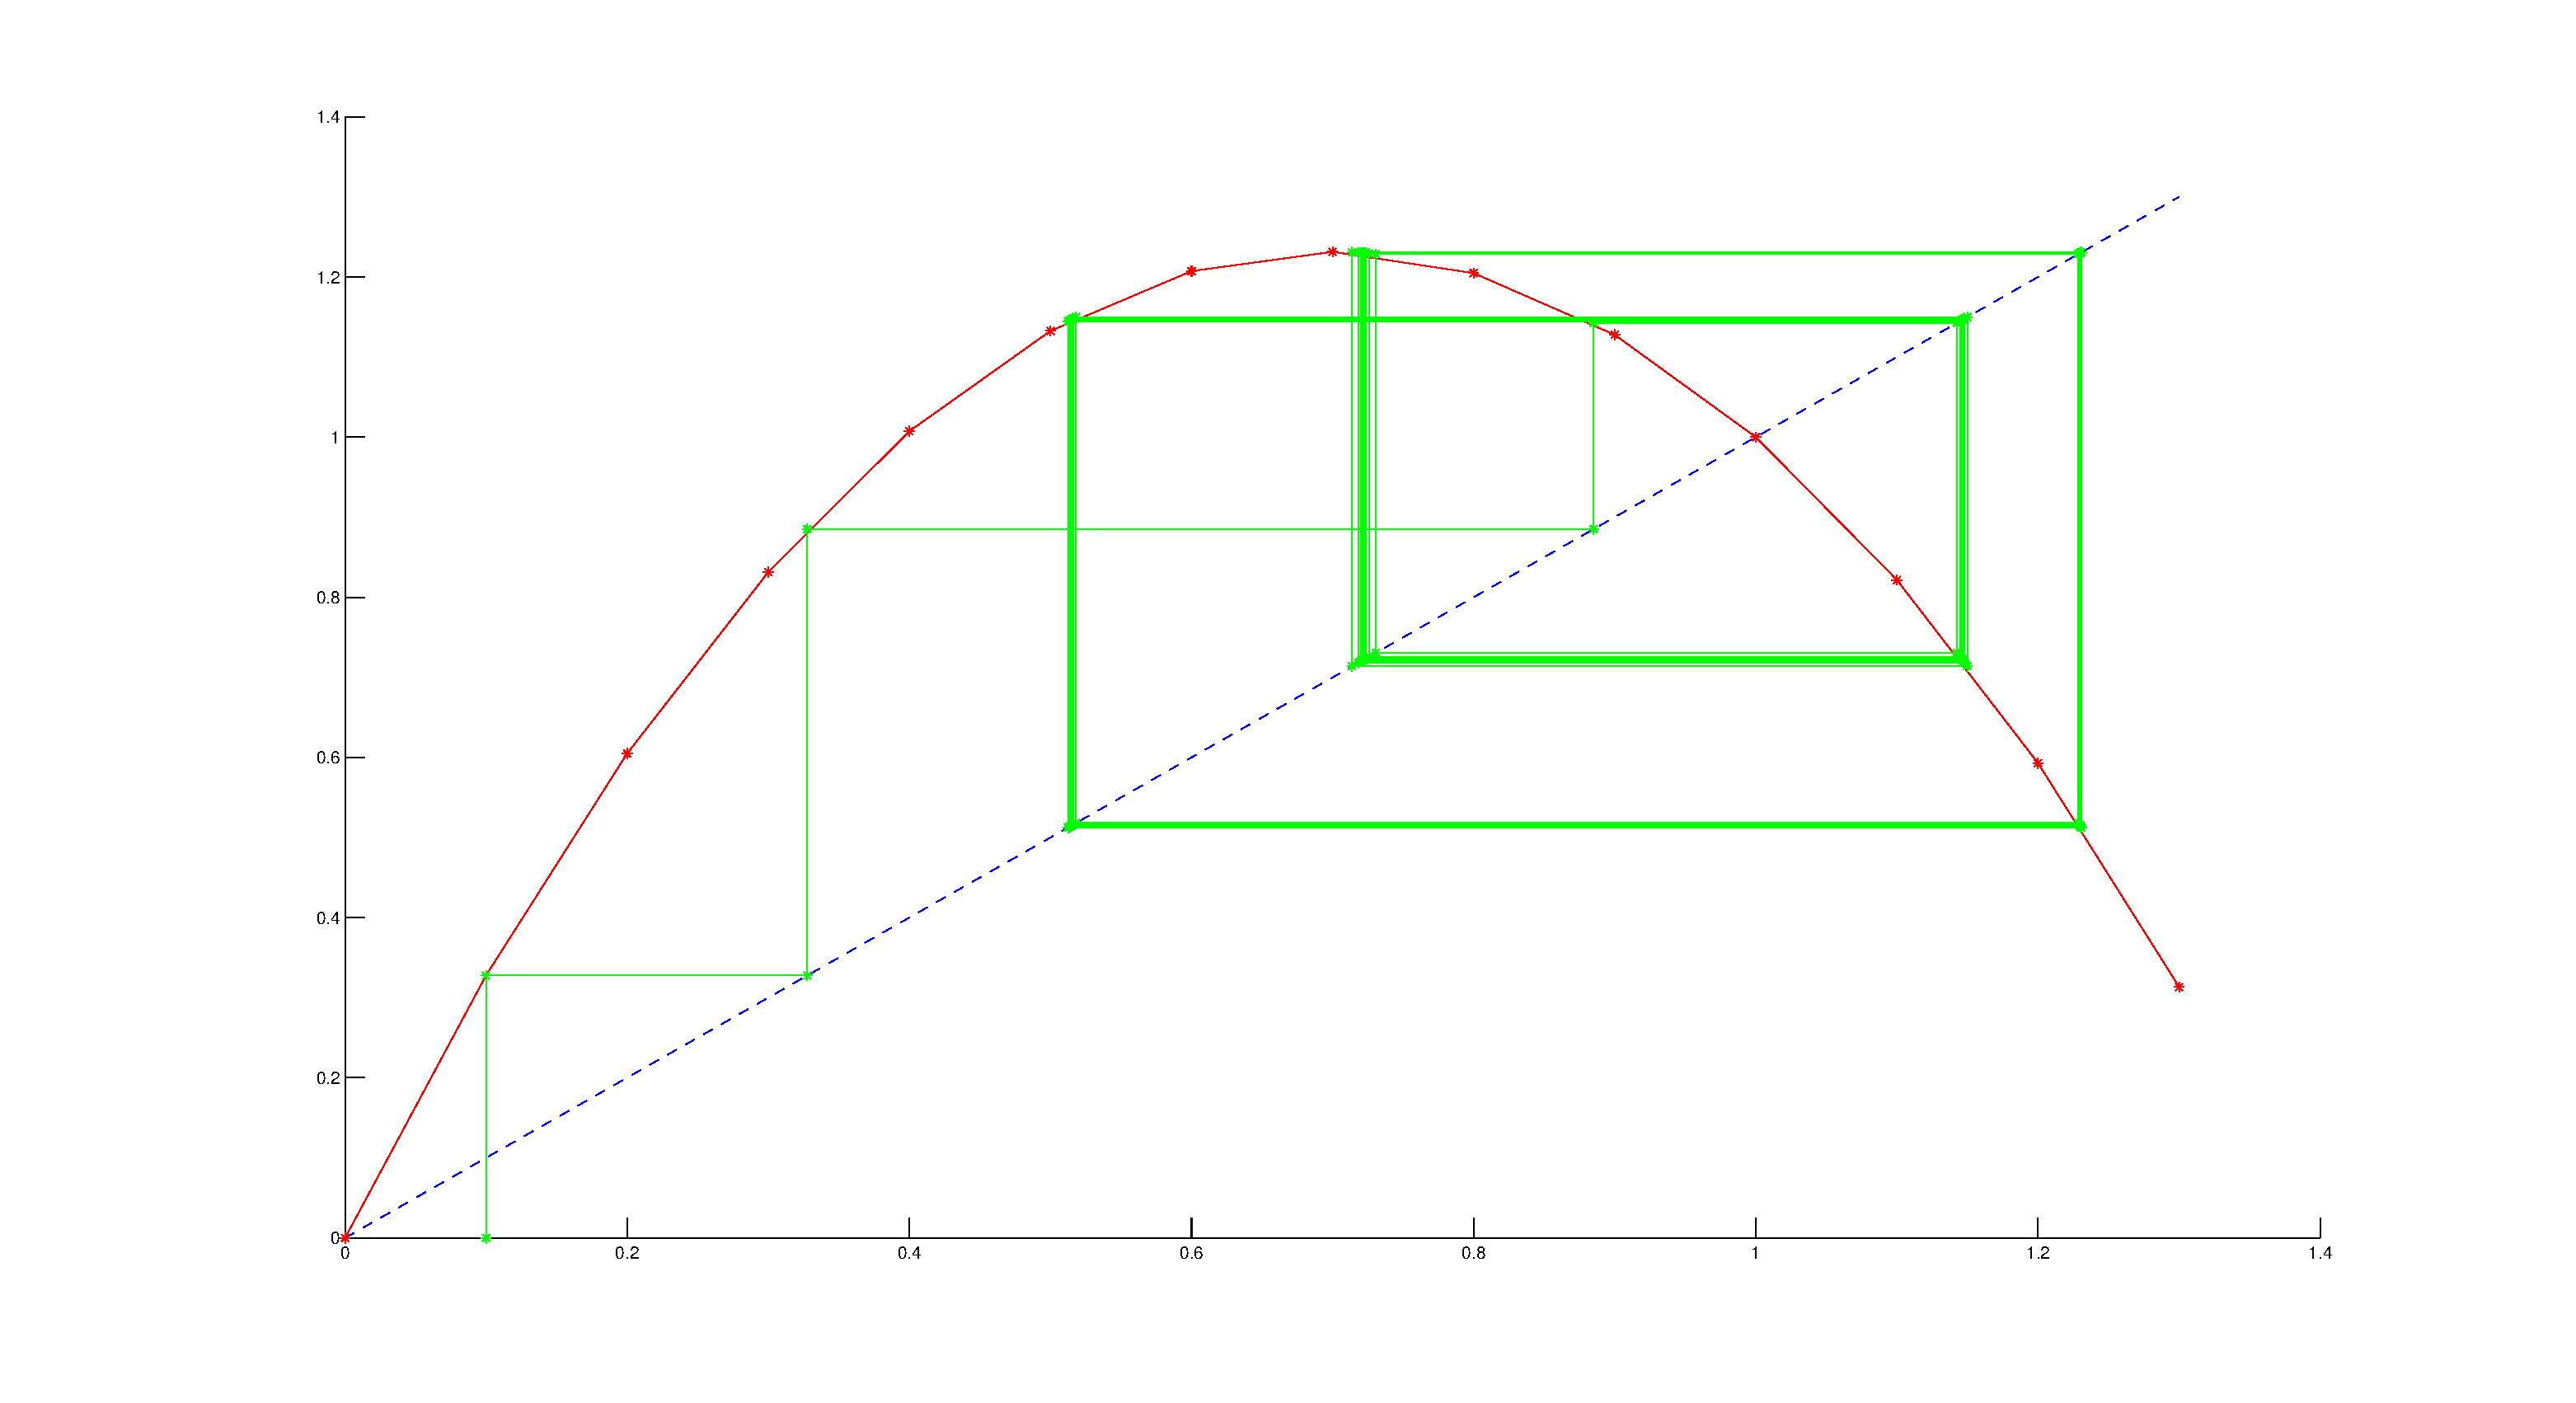
\includegraphics[width=\textwidth]{EPSFiles/CobwebPD_4_VMap}
                \caption{4 Attractors, \newline r = 2.53}
                \label{fig:Cobweb4}
        \end{subfigure}
        \begin{subfigure}[b]{0.19\textwidth}
                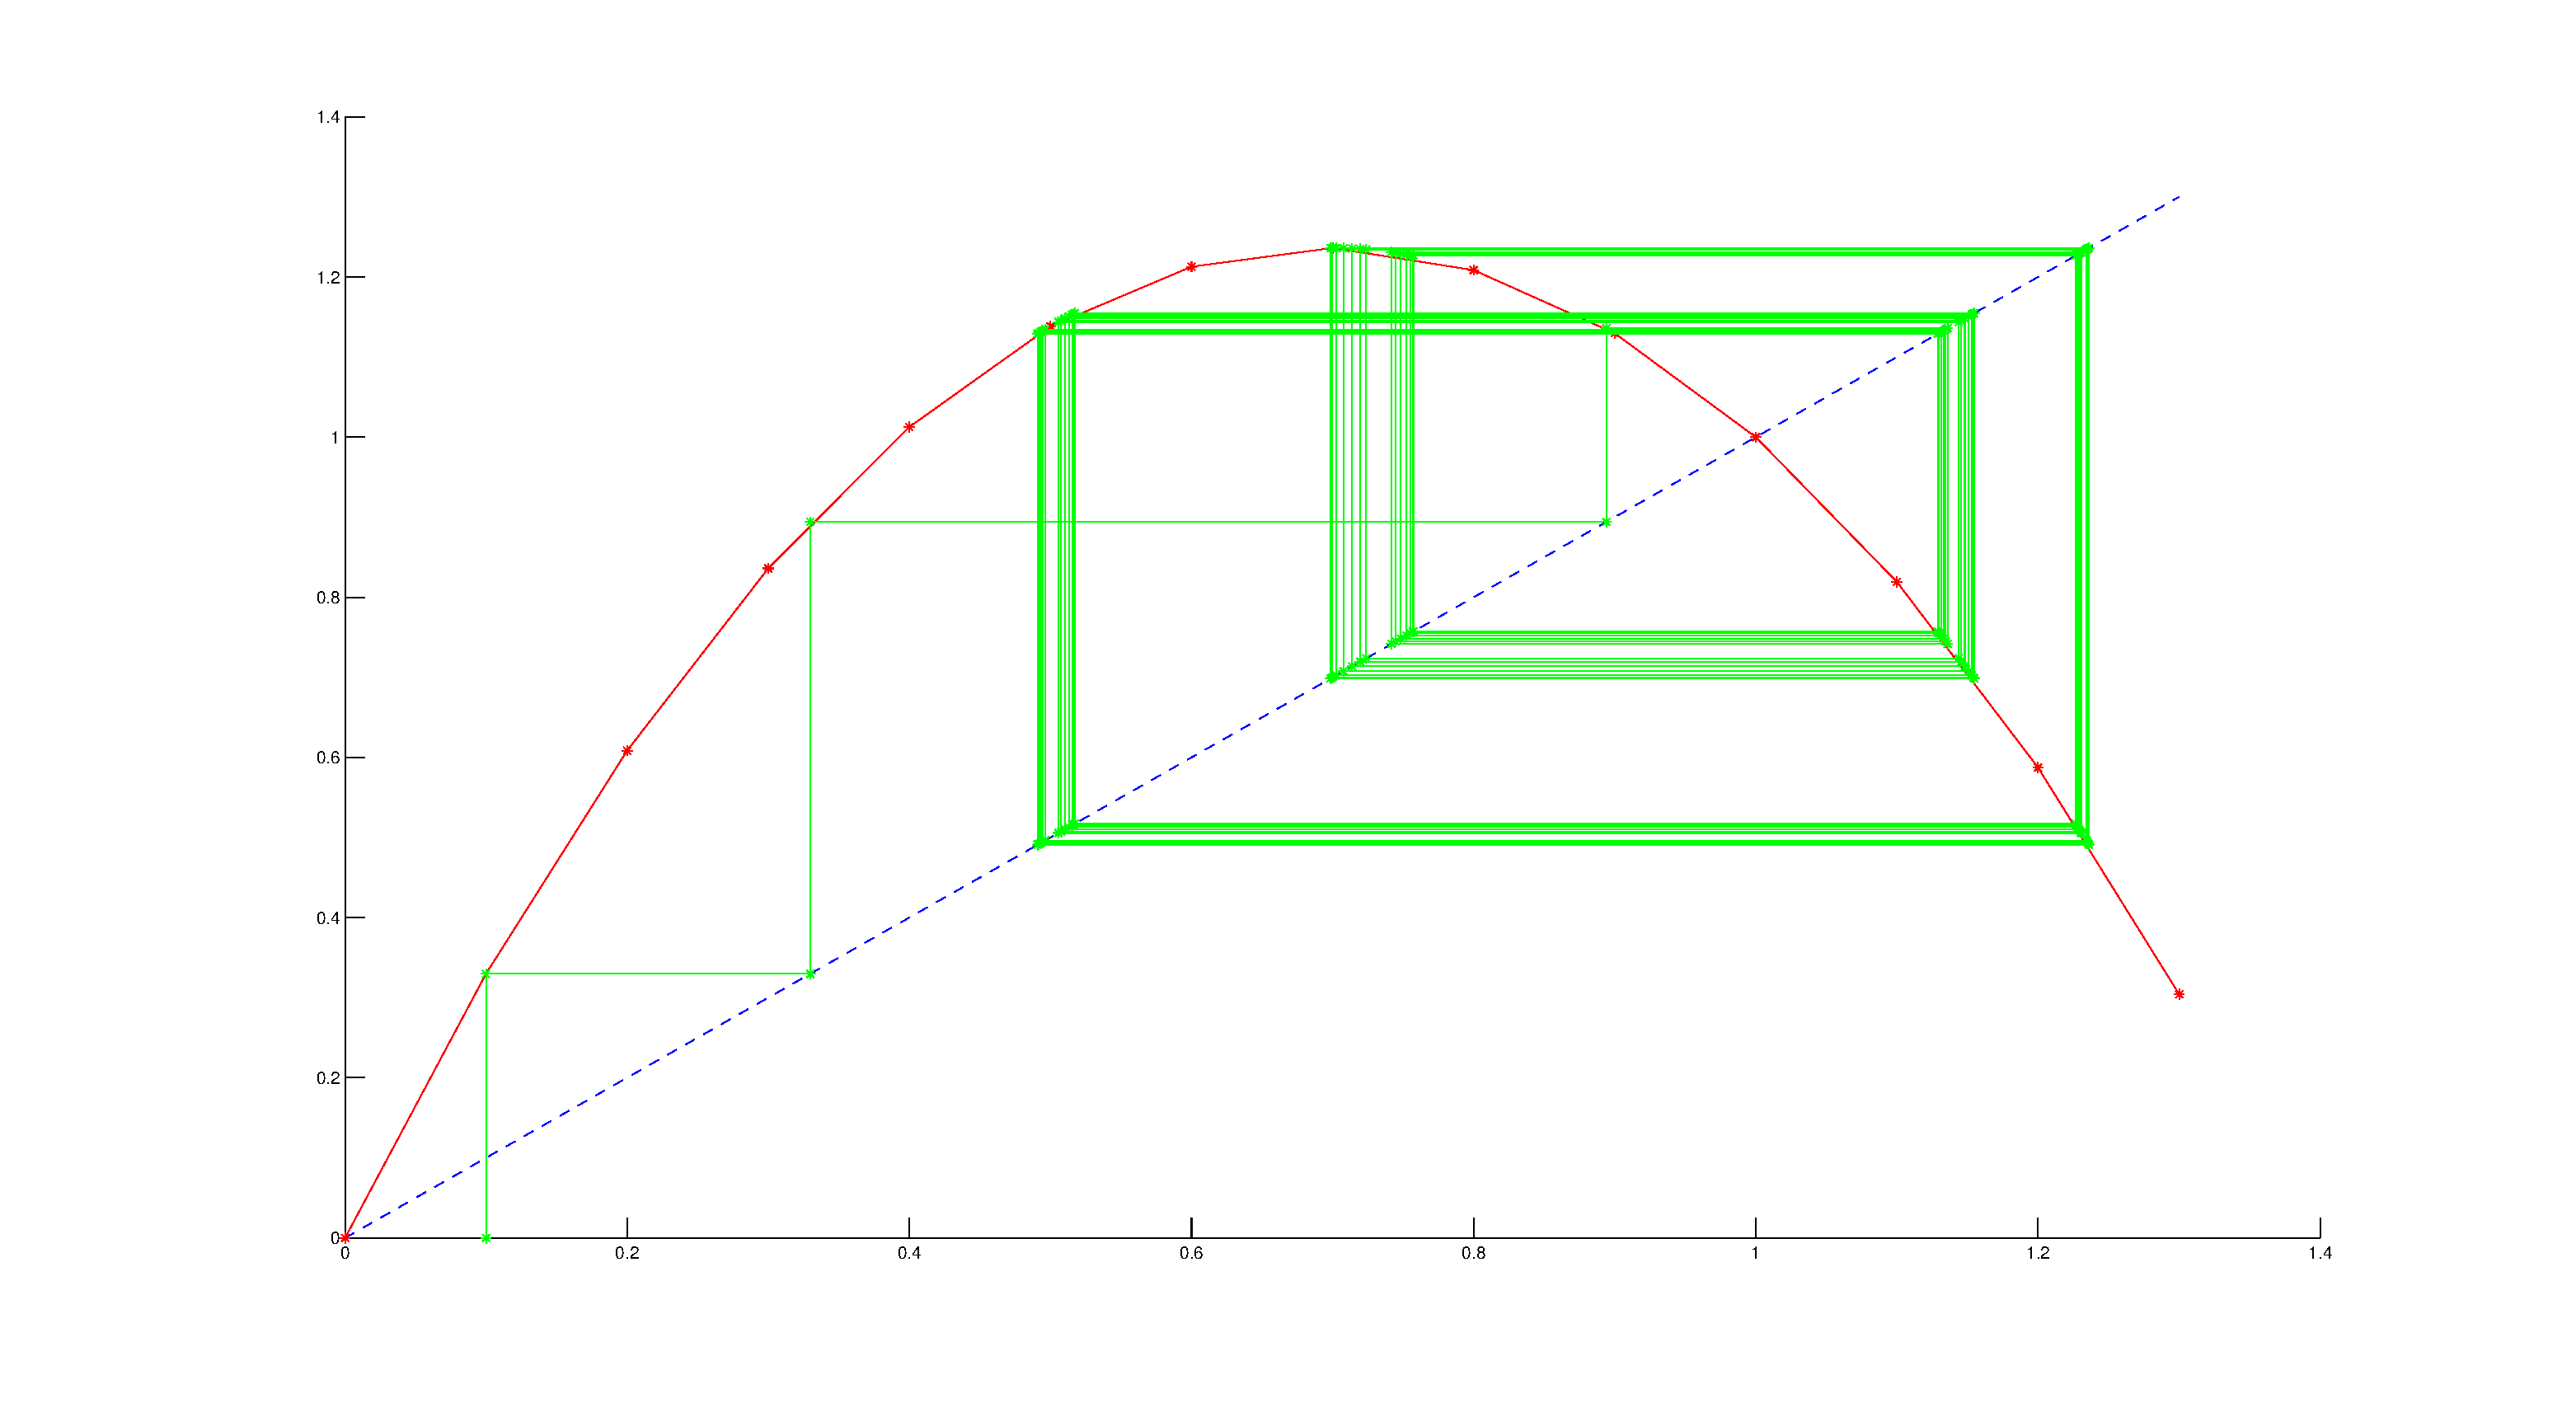
\includegraphics[width=\textwidth]{EPSFiles/CobwebPD_8_VMap}
                \caption{8 Attractors, \newline r = 2.553}
                \label{fig:Cobweb8}
        \end{subfigure}
        \begin{subfigure}[b]{0.19\textwidth}
                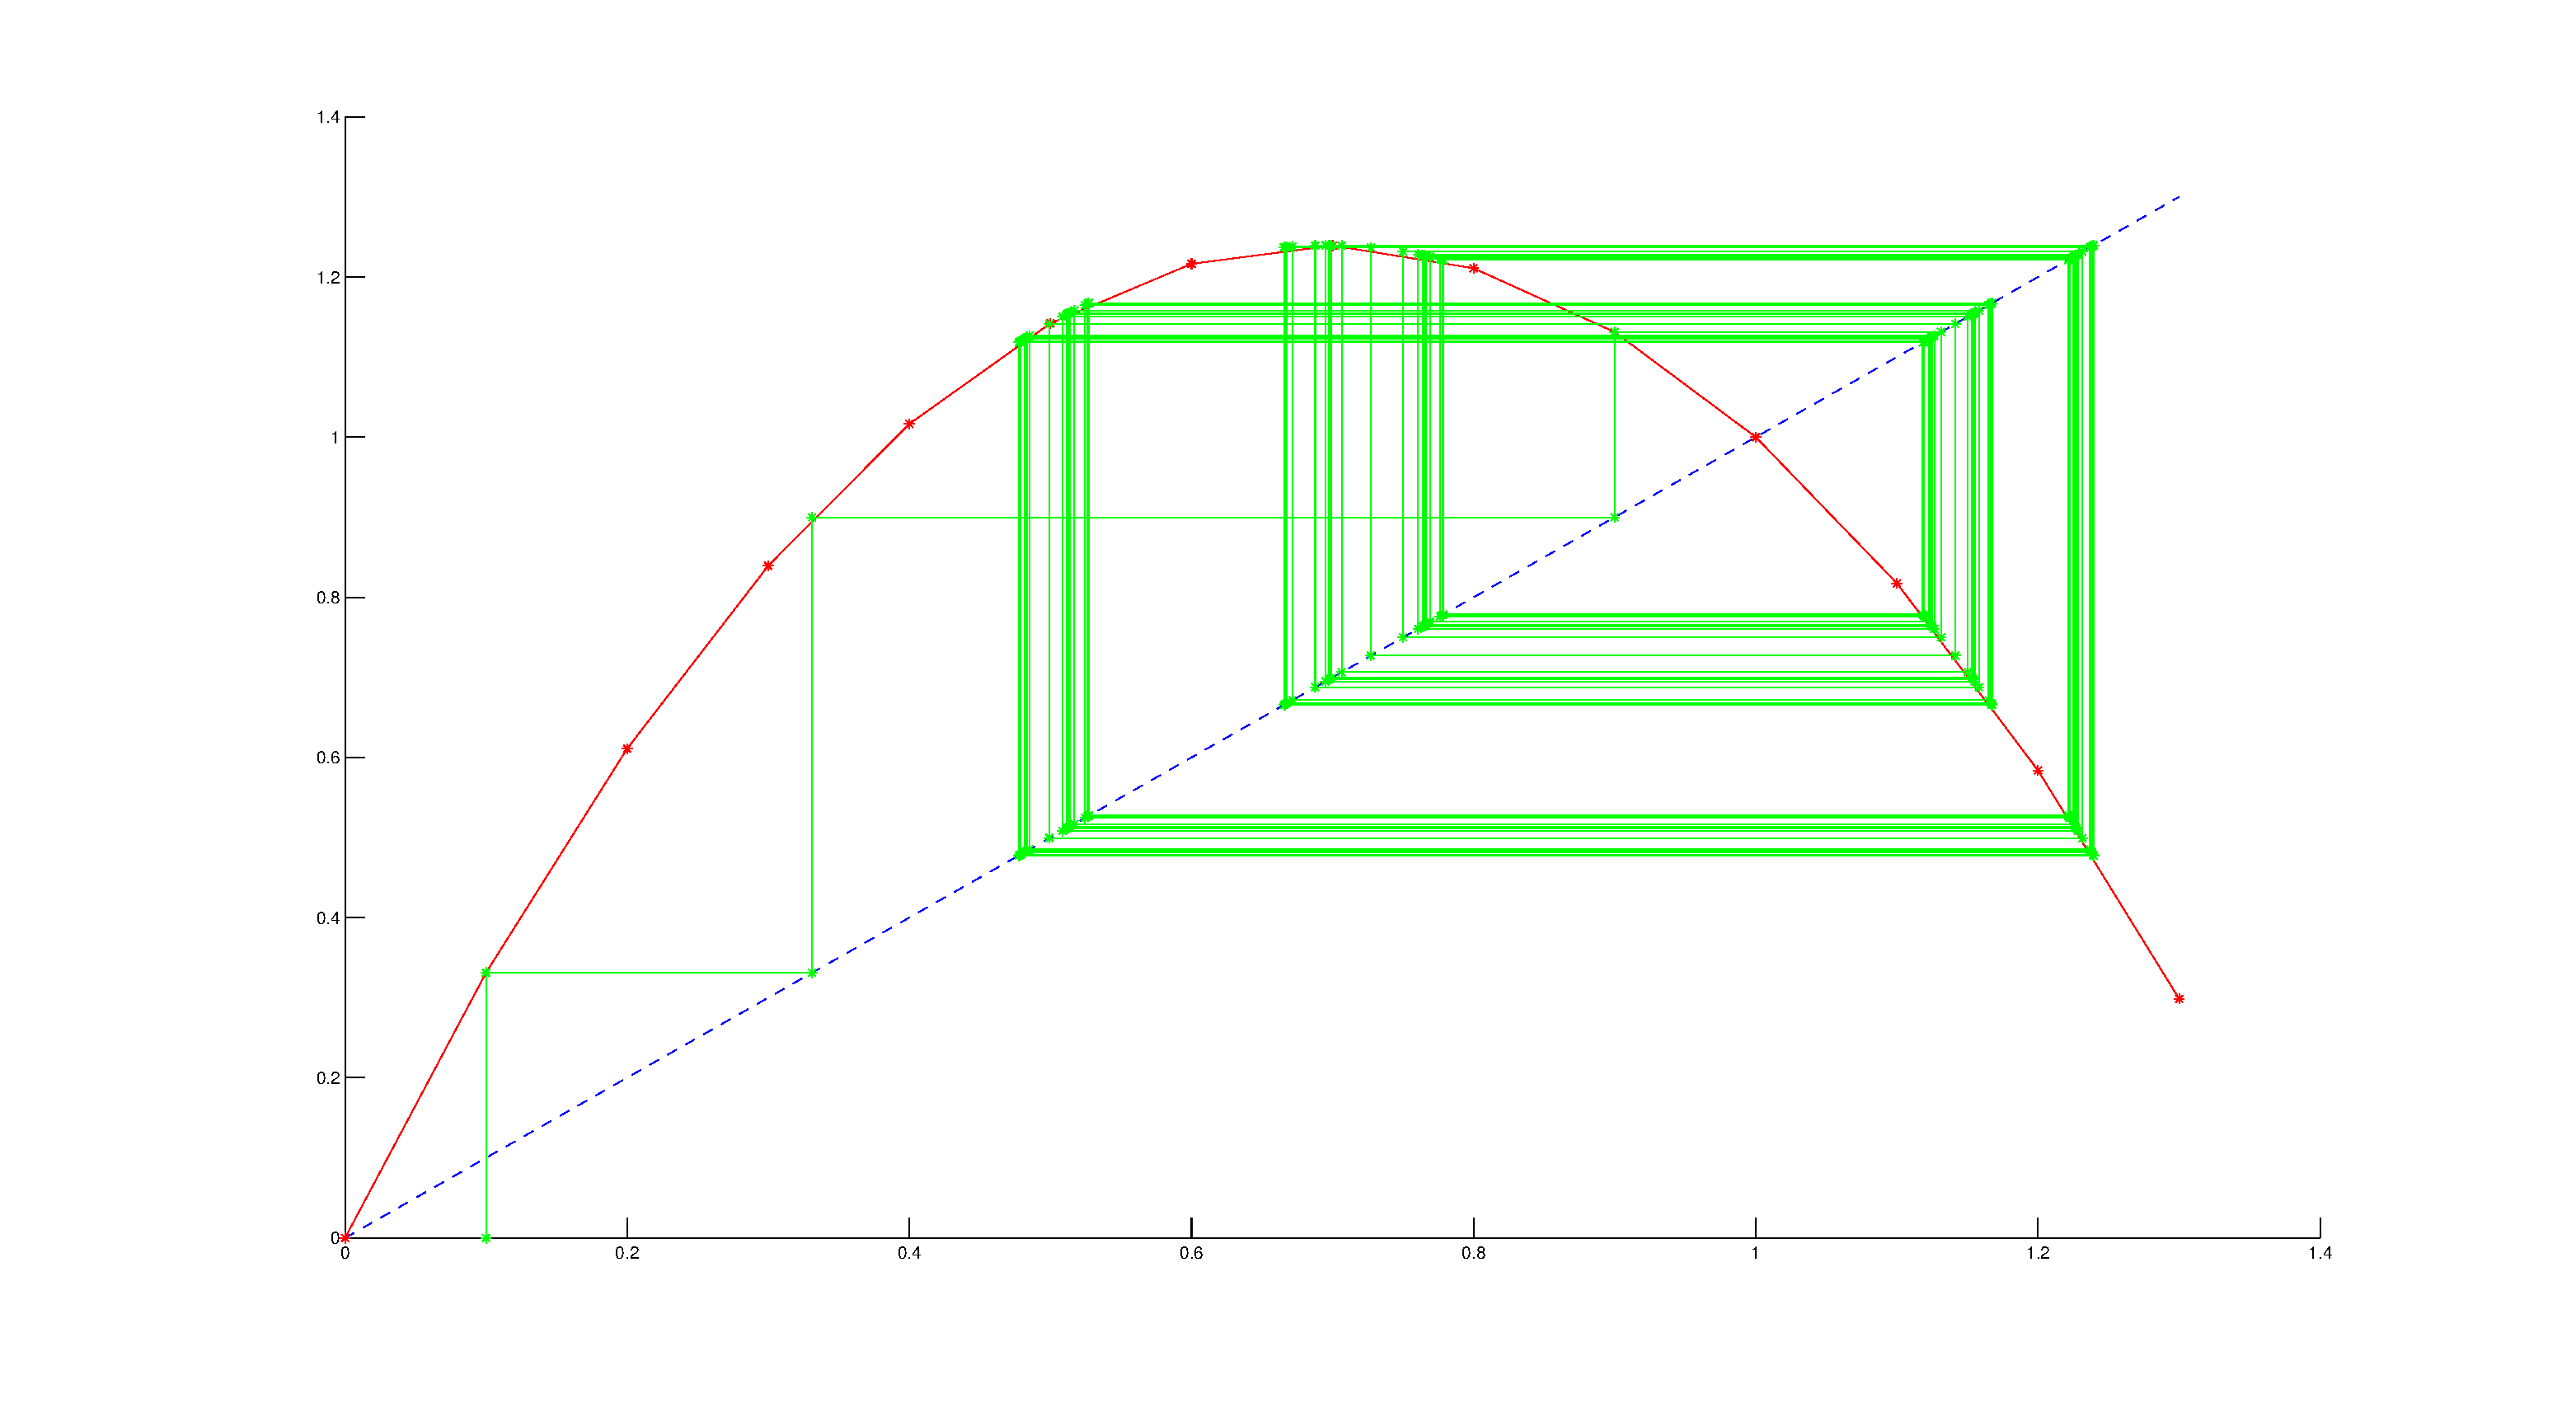
\includegraphics[width=\textwidth]{EPSFiles/CobwebPD_16_VMap}
                \caption{16 Attractors, \newline r = 2.568}
                \label{fig:Cobweb16}
        \end{subfigure}
        \begin{subfigure}[b]{0.19\textwidth}
                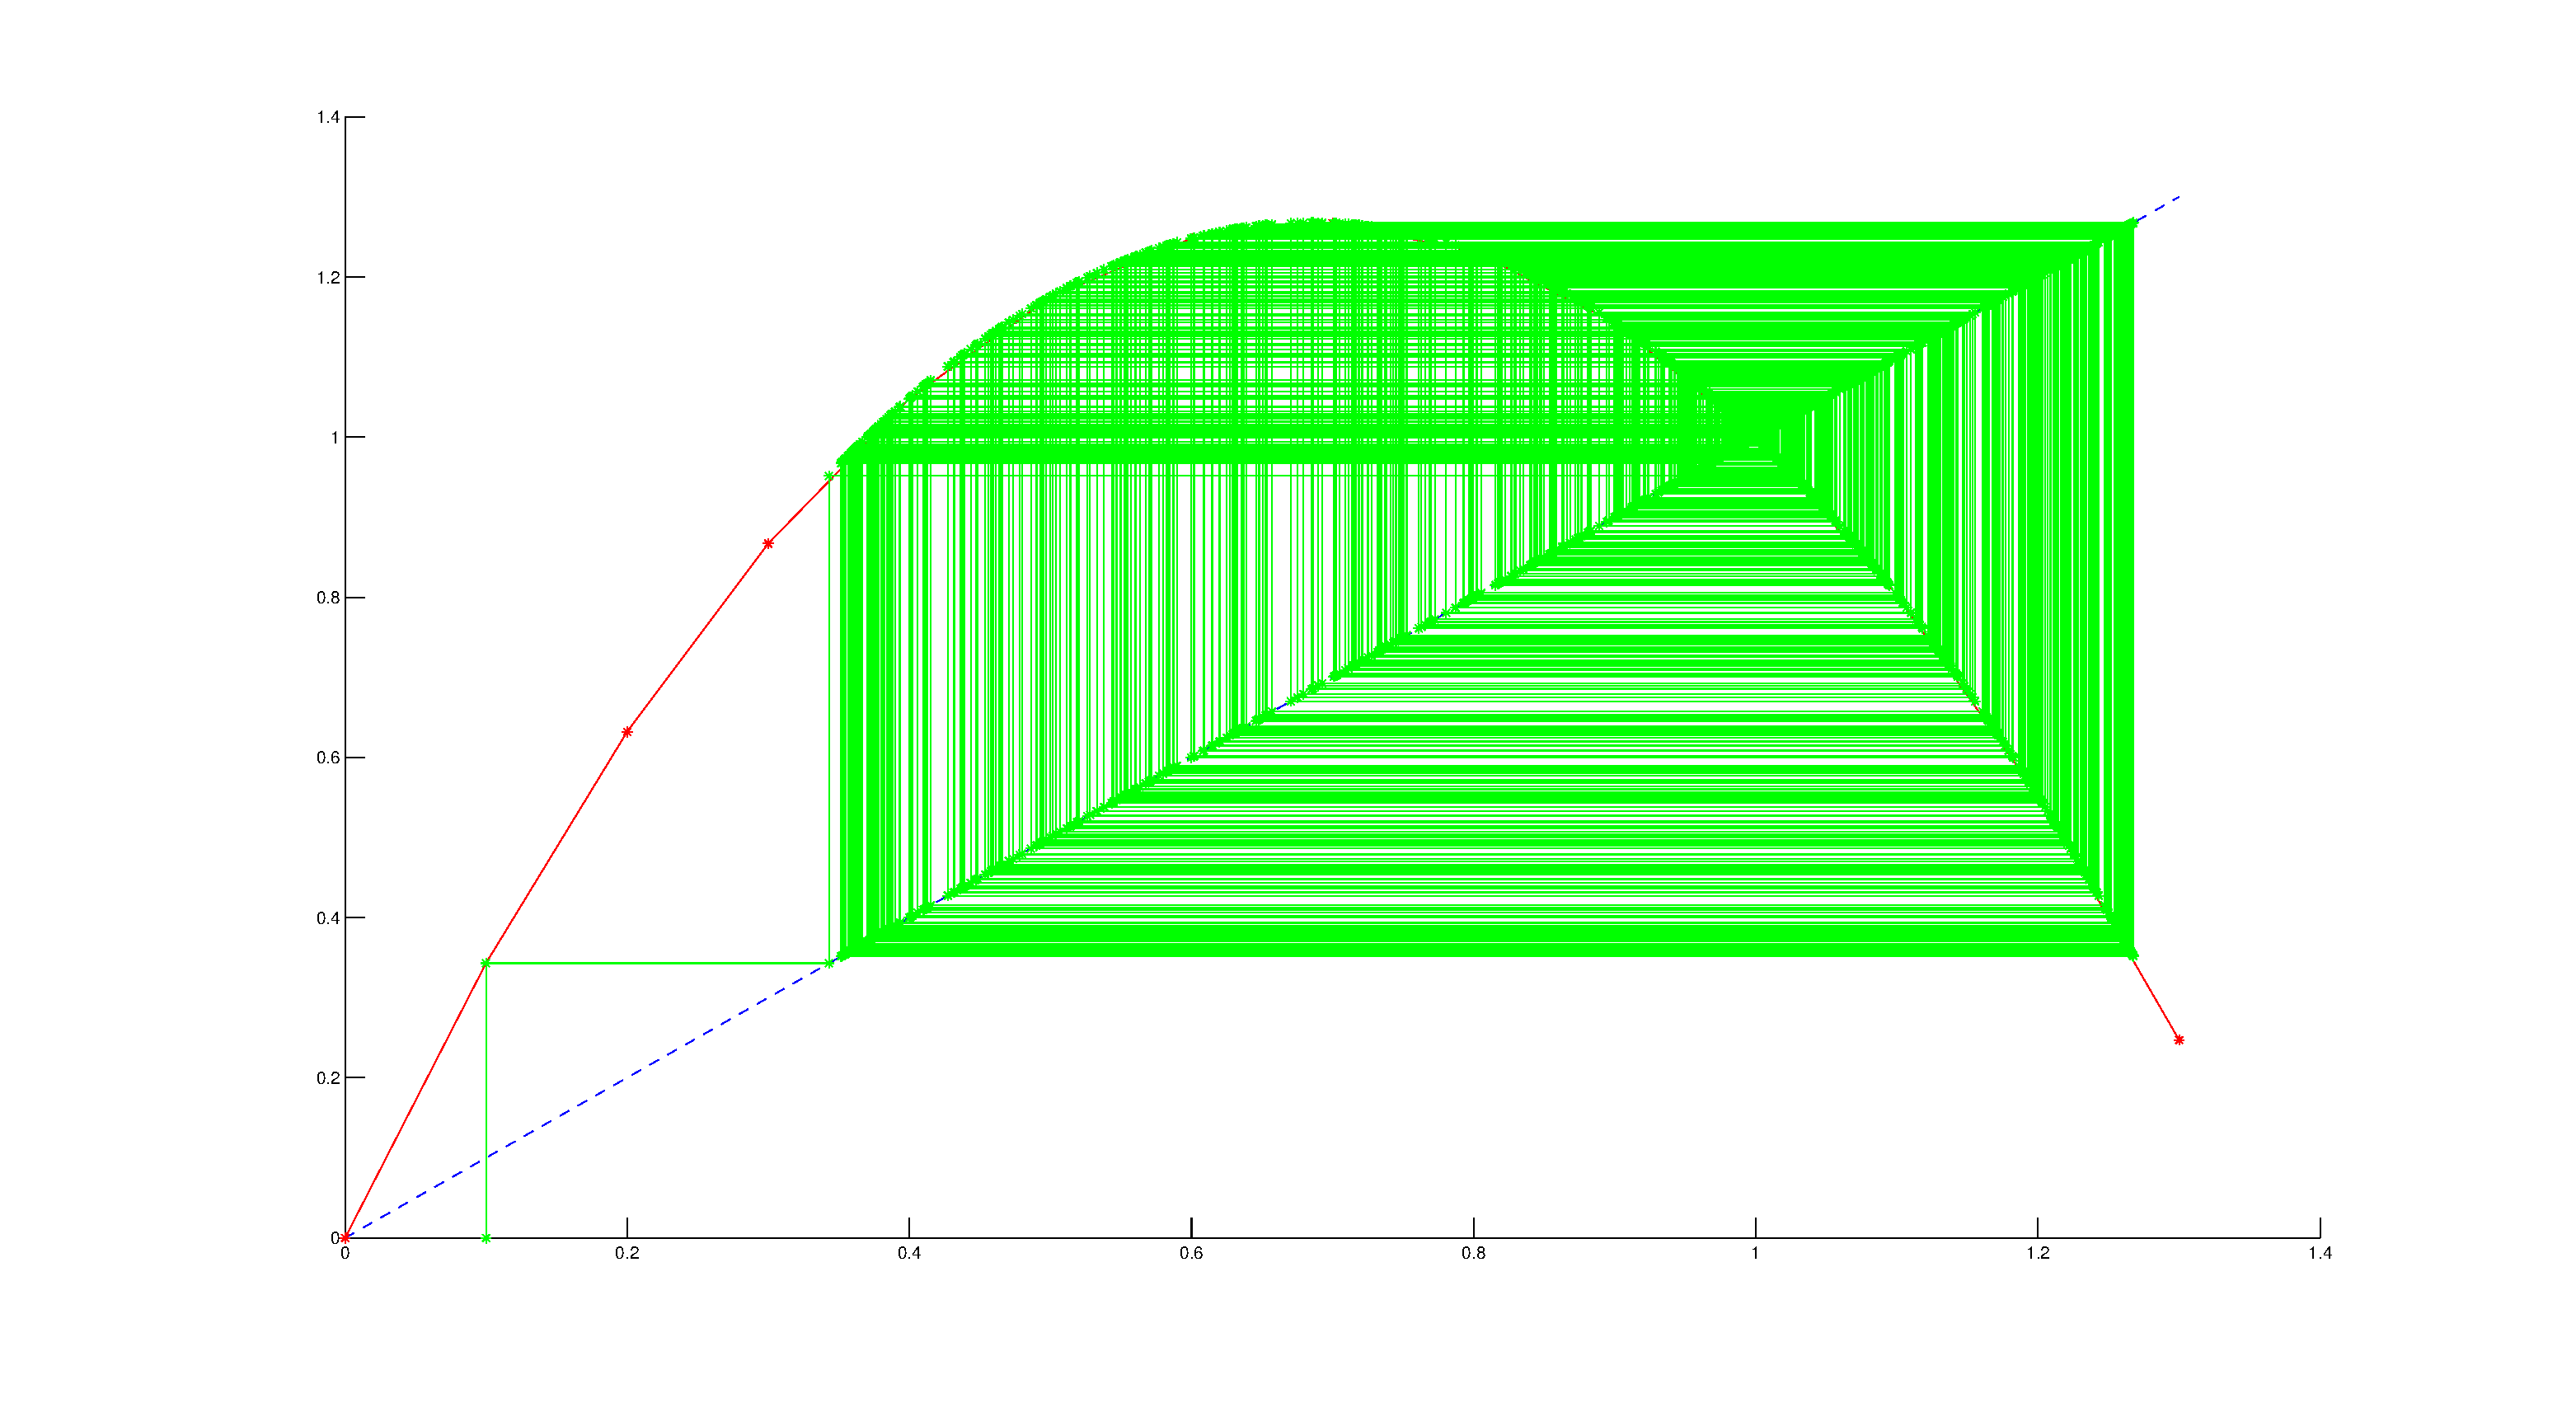
\includegraphics[width=\textwidth]{EPSFiles/CobwebPD_Random_VMap}
                \caption{Chaos, \newline r = 2.7}
                \label{fig:CobwebChaos}
        \end{subfigure}  
        \caption{Cobweb diagrams for Verhulst map with different $r \textrm{-values}$.}
\end{figure}

We found that different shaped orbits occurred at different r values corresponding to the number of
 period doubling points it has. You can see that a period double with two attractors shown in figure~\ref{fig:Cobweb2}
  looks like a rectangle orbit and a period double with four attractors in figure~\ref{fig:Cobweb4} is
   shown as two overlapping rectangles. When the amount of period doubling becomes quite large the shape of the
    orbits become more and more complex until it is hard to see  
     values being repeated and the orbit is filled with an infinite number of attractors scattered
      about the graph which depict a chaotic orbit. There still seems to be order amongst this chaos
       though.
 
The figure below is the result of plotting the points of the Verhulst map's $x_{k}$ values
 against the value of $r$ they were calculated at for $ 0 \leq r < 3 $. As you can see,  
  the graph seems to be covered up by lots of interweaving lines, however, looking closely,
   there seems to be a main pattern we are able to make out in the graph's ongoing structure.
    This figure shows the period doubling more clearly than the cobweb diagrams could.

\begin{figure}[H]

    \centering

    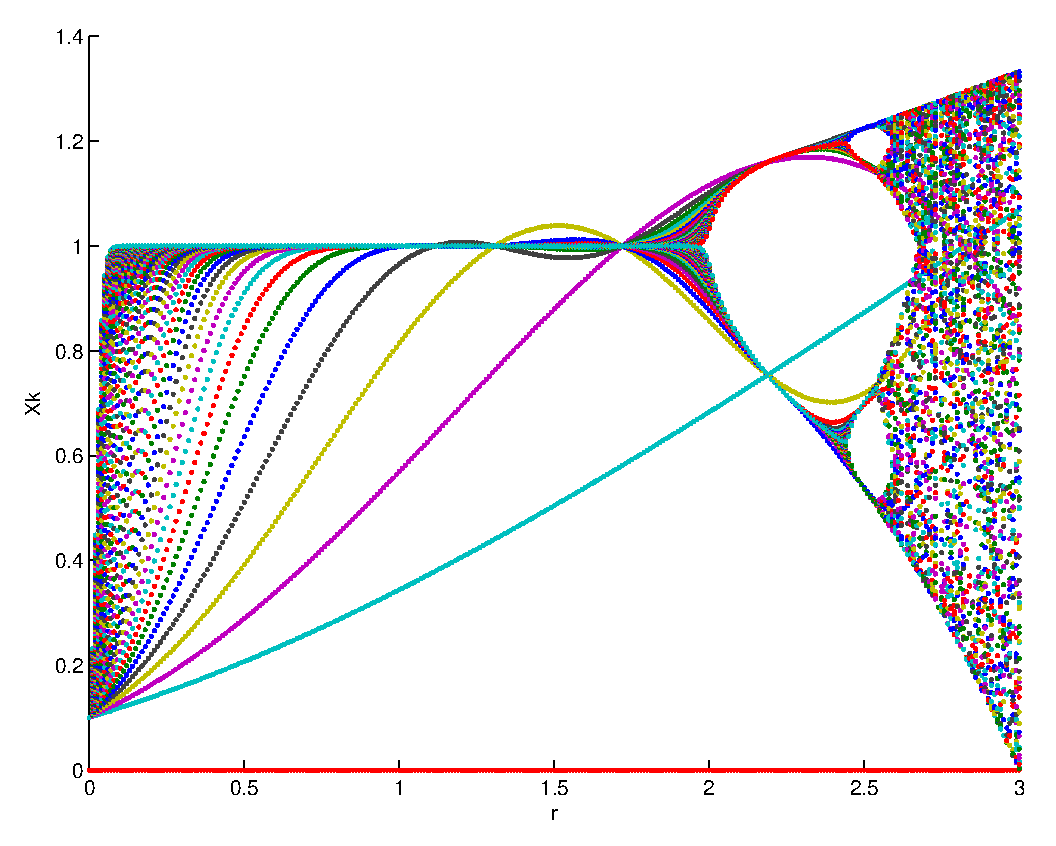
\includegraphics[scale=0.3]{EPSFiles/VerhulstAllXk}

    \caption{Verhulst map - plotting all iterations of $x_{k}$ against values of $r$ in range $0 \leq r < 3$.}
    \label{fig:VerhulstAllXk}

\end{figure}

The main pattern in the diagram above is therefore showing the value of the \emph{fixed points} in the
 Verhulst map for each $r$ value. Fixed points are the points that the map will converge to, if
  enough iterations are completed. These fixed points are also known
   as attractors, as mentioned before. The interweaving lines are simply the values of $x_{k}$ for
    very small k - before converging on the fixed points. Each colour in these figures corresponds to 
     a different iteration of $x_{k}$, so you can track what happens to each iteration as $r$ increases.

Period doubling becomes much clearer in the following two figures. The sequence of period doublings,
 or \emph{bifurcations}, as $r$ is varied is known as a \emph{period doubling cascade}. If the number
  of attractors at a given $r \textrm{-value}$ is \emph{n}, we say that there is a \emph{n-cycle
   attractor} for that value of $r$.

\begin{figure}[H]

    \centering

    \includegraphics[scale=0.3]{EPSFiles/VerhulstDots}

    \caption{Verhulst map with $ x_{0} = 0.1 $. $0 \leq r < 3$.}
    
    \label{fig:VerhulstDots}

\end{figure}

The figure above is created on Matlab by only plotting the values of $x_{k}$ for large $k$,
 thus getting rid of the interweaving lines shown in figure~\ref{fig:VerhulstAllXk}, which were caused by also plotting the $x_{k}$ for small $k$, when it hadn't
   converged on an attractor yet. In the above figure, only the final 32 iterations
    out of 10000 iterations of $x_{k}$ are plotted for each $r \textrm{-value}$. 

%It turns out that, for example, during a 2-cycle, the value of $x_{k}$ will oscillate between the 2
 %attractors, so odd iterations, i.e. $x_{1}$, $x_{3}$, etc., will all converge to one of the
  %attractors, and the even iterations will converge to the other one. This can be generalised to any n-
  %cycle, as consecutive iterations will go through attractor 1, then attractor 2, and so on, until
  % attractor $n$, which will be followed by attractor $1$, and then the pattern repeats itself\cite{Verhulst
  %  Map Period Doubling Information}. This idea is used in the code that finds the points where period
  %   doubling occurs, shown in the figure below.

%The point at $r = 0$ is due to the fact that, at $r = 0$, the equation simply
% becomes $x_{k + 1} = x_{k}$. Since the initial value for x was 0.1, in this case,
%  all iterations will give $x_{k} = 0.1$ when $r = 0$. 

The period doubling begins at $r = 2$, and after that, the distance between
 consecutive period doubling points on the $r \textrm{-axis}$ keeps decreasing. As
  $r$ increases to 2.57, this distance between consecutive period doubling points
   tends to 0. Eventually, at r = 2.57, there will be infinitely many attractors, so
    the value of each $x_{k}$ is essentially random\cite{Verhulst Map Period Doubling Information}. It is at this $r \textrm{-value}$
     that the Verhulst map descends into chaos. For $r > 3$, there are no attractors, 
      as $x_{k}$ now diverges for all $r \textrm{-values}$ above three.

This may all seem quite unexpected already - that such a simple equation can result
 in such a complex structure, simply by varying a single parameter. However, what is
  even more intriguing is the fact that inside the chaos, inside the \emph{randomness}, 
   order arises. Notice the point at about $r = 2.828$, there are 
    three attractors in the middle of the chaotic mess. This order doesn't last very long, and as
     $r$ increases, it quickly descends into chaos again, but the fact that it appears at all is
      extraordinary. 

%REFERENCE SOMETHING FROM GLEICK BOOK???

%TALK ABOUT HOW I DID THIS (On MATLAB)

\begin{figure}[H]

    \centering

    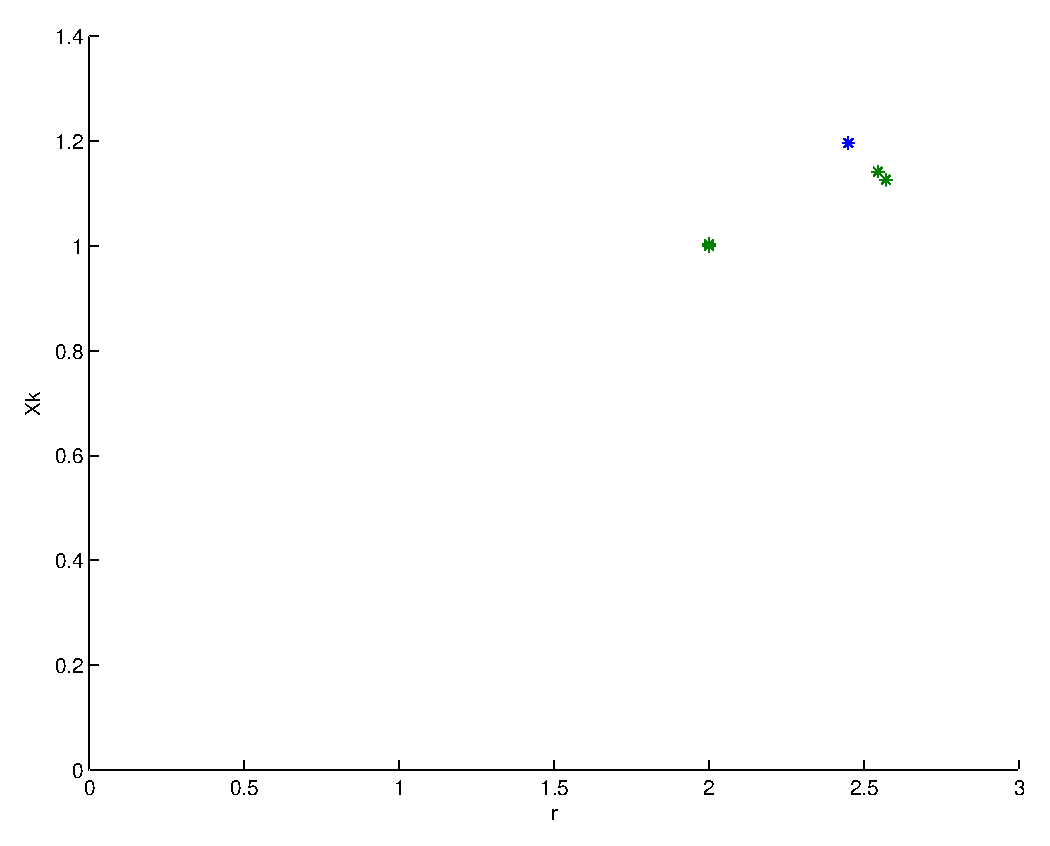
\includegraphics[scale=0.2]{EPSFiles/MAINVerhulstPointsEPS}

    \caption{The $r \textrm{-values}$ on the Verhulst map, from figure~\ref{fig:VerhulstDots}, where period doubling occurs.}
    
    \label{fig:VerhulstPoints}

\end{figure}

The figure above shows the first four values of $r$ where the period doubling occurs
 - 2, 2.449, 2.544, and 2.569. As you can tell, this is getting closer and closer to
  a particular number, namely 2.57, the point at which chaos occurs. Whilst analysing
   these points we found that the ratios of the differences between them also tended to a 
   	limit, this limit seemed close to the constant found by Mitchell Feigenbaum that occurs in
   	 many other non-linear maps\cite{Verhulst Map Period Doubling Information}. From the accuracy of the period doubling points we obtained, we didn't find exact convergence to the Feigenbaum constant, however the calculations below roughly show that the values of two ratios of differences are close to this constant. Finding more points of bifurcation would have given more accurate values for this ratio.	 
   	  
\begin{center} 	  
   	  $\frac{(2.449-2)}{(2.544-2.449)} = 4.726315$, $\frac{(2.544-2.449)}{(2.569-2.544)} = 3.8$ 
\end{center}
 
%FEIGENBAUM CONSTANT (Verhulst 2.57 google books- Feigenbaum's coming :P (Kiran))
At first we tried to create the figures in Matlab by always starting with $x_{0} = 0.1$, and then plotting the values of $x_{k}$
  when the number of iterations gets bigger than a certain value. This seemed to be time 
   consuming when we started making the interval between each consecutive $r \textrm{-value}$ smaller. It seemed 
    to be more efficient to create an array of values for large $x_{k}$ and then plot the whole 
     array against its' $r \textrm{-value}$ instead. 
       This method was carried through when making the plots for the other logistic maps. Other ways we 
 improved the figures for the non-linear maps were increasing the precision, by incrementing $r$ by a
  smaller amount so that the figure had more detail, and by making the array to store the iterations of
   $x_{k}$ large enough to store them all, rather than making a small array and having it increase in
    size every time it needed to be bigger, because this involved copying all contents of the array of
     size $n$ over to another array of size $n + 1$. Furthermore, we got rid of magic numbers by giving
      most parameters variable names, so that the figure can be easily improved or changed to be
       slightly different.
       
For figure~\ref{fig:VerhulstPoints}, showing only the first points where period doubling occurs, we made a $\lambda$
 variable, to help detect when the values of $x_{k}$, that are $\lambda$ iterations apart, start to be
  different, as opposed to having exactly the same value. When they have the same value, it means
   they are converging to the same attractor, and this $r \textrm{-value}$ produces a $\lambda \textrm{-cycle}$. When they start to have a different value, found by
    checking to see if $10^{-8} < |x_{k_{2}} - x_{k_{1}}| < 10^{-3}$, this means period doubling has
     just occurred. The inequality used shows that if the points get more than $10^{-3}$ apart, they
      won't be plotted, so the points after period doubling occurs will not be plotted. $\lambda$ starts at 2, so it checks for a 2-cycle, and then $\lambda$ is multiplied by 2 on each iteration of the loop, until $\lambda$ is large enough.
 
The initial value of $x$ in figures~\ref{fig:VerhulstDots} and~\ref{fig:VerhulstPoints} is 0.1. The 6 subfigures below show the effect of changing the initial $x \textrm{-value}$. For $ 0 < x_{0} < 1 $, the
 bifurcation diagram doesn't really change. The only thing that changes here is that
  some of the iterations of $x_{k}$ move around a bit, although the attractors stay
   the same. As an example, during a four-cycle attractor, $x_{0} = 0.1$ may mean
    that $x_{254}$ is on the attractor with the highest value, and $x_{255}$ is on
     the attractor with the lowest value. With another $x_{0}$, with 
      $0 < x_{0} < 1$, such as $x_{0} = 0.4$, $x_{254}$ may now be on the attractor
       with the second highest value, and $x_{255}$ may now be on the top attractor.
        Also, the points in the chaotic section move about seemingly randomly as
         $x_{0}$ is varied in this range. However, the shape of this diagram is kept the  same in this range of $x_{0}$ values. 
     For $x_{0} = 0$, the whole diagram is just a straight horizontal line, with all
 $x_{k}$ equal to 0, which is fairly obvious when looking back at the recursive equation
  defining the map. The same sort of thing can be said for $x_{0} = 1$, where the
   whole diagram is, again, just a straight horizontal line, but this time with all
    $x_{k}$ equal to 1. 
   Varying the initial $x$ value really starts to get interesting when $x_{0} > 1$.
 This is because as $x_{0}$ increases, while in this range, the diagram begins to stop
  plotting any attractors for the larger $r \textrm{-values}$ - The domain of the
   bifurcation diagram begins to decrease as $r$ increases above 1, which can be seen in the 6
    subfigures below. This decreasing of the domain happens because, as $x_{0}$
     increases, the smallest $r \textrm{-value}$ that causes $x_{k}$ to 
      diverge, and thus have no attractors, decreases. 

\begin{figure}[H]
        \centering
        \begin{subfigure}[b]{0.2\textwidth}
                \includegraphics[width=\textwidth]{EPSFiles/VerhulstDots}
                \caption{$x_{0} = 0.1$}
                \label{fig:Verhulst0.1}
        \end{subfigure}
        \begin{subfigure}[b]{0.2\textwidth}
                \includegraphics[width=\textwidth]{EPSFiles/Verhulst05}
                \caption{$x_{0} = 0.5$}
                \label{fig:Verhulst0.5}
        \end{subfigure}
        \begin{subfigure}[b]{0.2\textwidth}
                \includegraphics[width=\textwidth]{EPSFiles/Verhulst1Improved}
                \caption{$x_{0} = 1$}
                \label{fig:Verhulst1}
        \end{subfigure}
        
        \begin{subfigure}[b]{0.2\textwidth}
                \includegraphics[width=\textwidth]{EPSFiles/Verhulst13}
                \caption{$x_{0} = 1.3$}
                \label{fig:Verhulst1.3}
        \end{subfigure}
        \begin{subfigure}[b]{0.2\textwidth}
                \includegraphics[width=\textwidth]{EPSFiles/Verhulst14Improved}
                \caption{$x_{0} = 1.4$}
                \label{fig:Verhulst1.4}
        \end{subfigure}  
        \begin{subfigure}[b]{0.2\textwidth}
                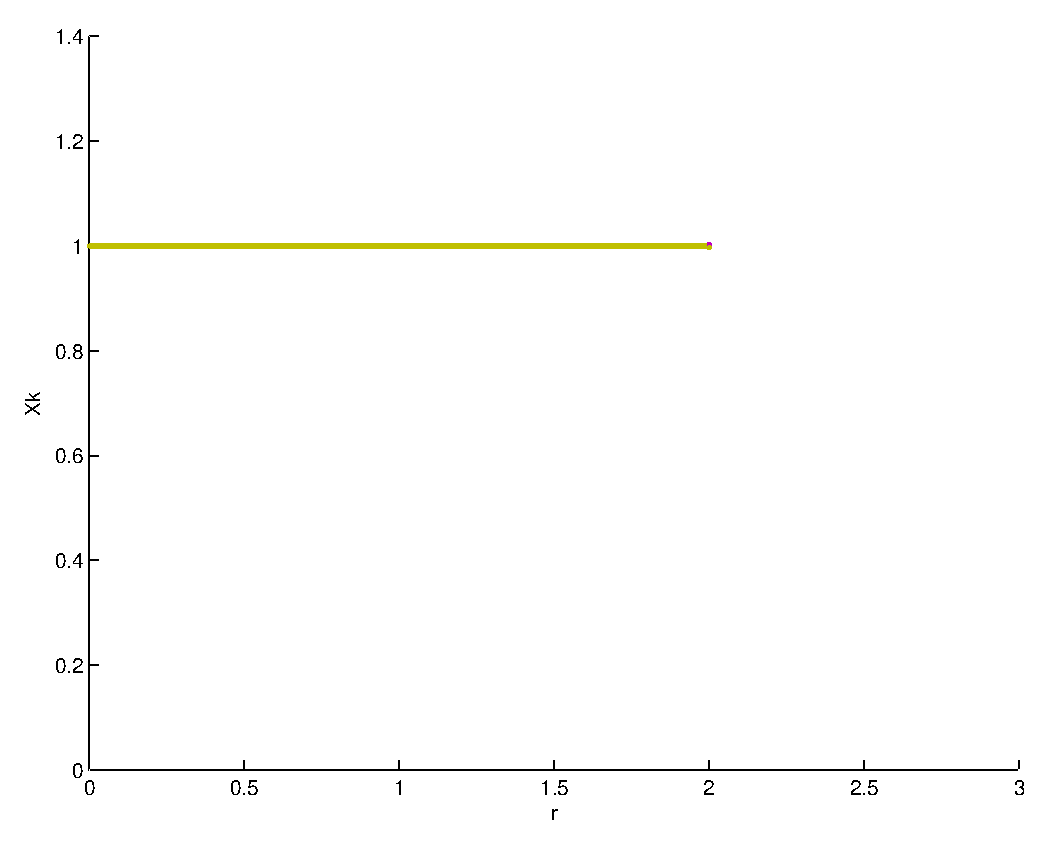
\includegraphics[width=\textwidth]{EPSFiles/Verhulst15}
                \caption{$x_{0} = 1.5$}
                \label{fig:Verhulst1.5}
        \end{subfigure}  
        \caption{Changing initial $x$ value for Verhulst map.}
\end{figure}

%DEPENDENCE ON INITIAL CONDITIONS SHOWN BY $0 < x_{0} < 1$ (Very Nice-(Kiran))
The fact that even the slightest change in $x_{0}$ changes the resulting figure shows that there is a
 strong \emph{dependence on the initial conditions}. Even the smallest change can have an effect, and,
  though this change may not seem like much at first, as more and more iterations are carried out, the
   initial condition seems to have more and more of an effect. This is known as the \emph{butterfly
    effect}\cite{Butterfly Effect}.

\subsection{Logistic Map}

The Verhulst map shown above is a specific form of the \emph{logistic map}, which
 has many forms. Another form of this logistic map, which will be investigated in
  this section, is defined by:

\[
  x_{k+1} = rx_{k}(1 - x_{k}) \textrm{, for \emph{k}} \geq 0
\]

%As a point of interest, nobody is quite sure why it is called the logistic map. In 1844, Pierre Verhulst,
% in one of his papers, \emph{Recherches mathématiques sur la loi d'accroissement de la population},
%  coined the term 'logistic equation' by naming his proposed differential equation a 'courbe logistique'
%   (A logistic curve)\cite{Pierre Verhulst Biography}. 

%TALK ABOUT ROBERT MAY IN CHAOS GLEICK BOOK POPULARISING LOGISTIC MAP

The figure below is the result of plotting the points of the Logistic map against $r$ for $0 \leq r < 4$.
 The result is largely the same as the corresponding figure for the Verhulst map. %TALK ABOUT ANY DIFFERENCES WITH INTERWEAVING LINES

%MAY NOT NEED THIS FIGURE AND TALK OF INTERWEAVING LINES FOR LOGISTIC IN REPORT BECAUSE IT IS SAME AS VERHULST

\begin{figure}[H]

    \centering

    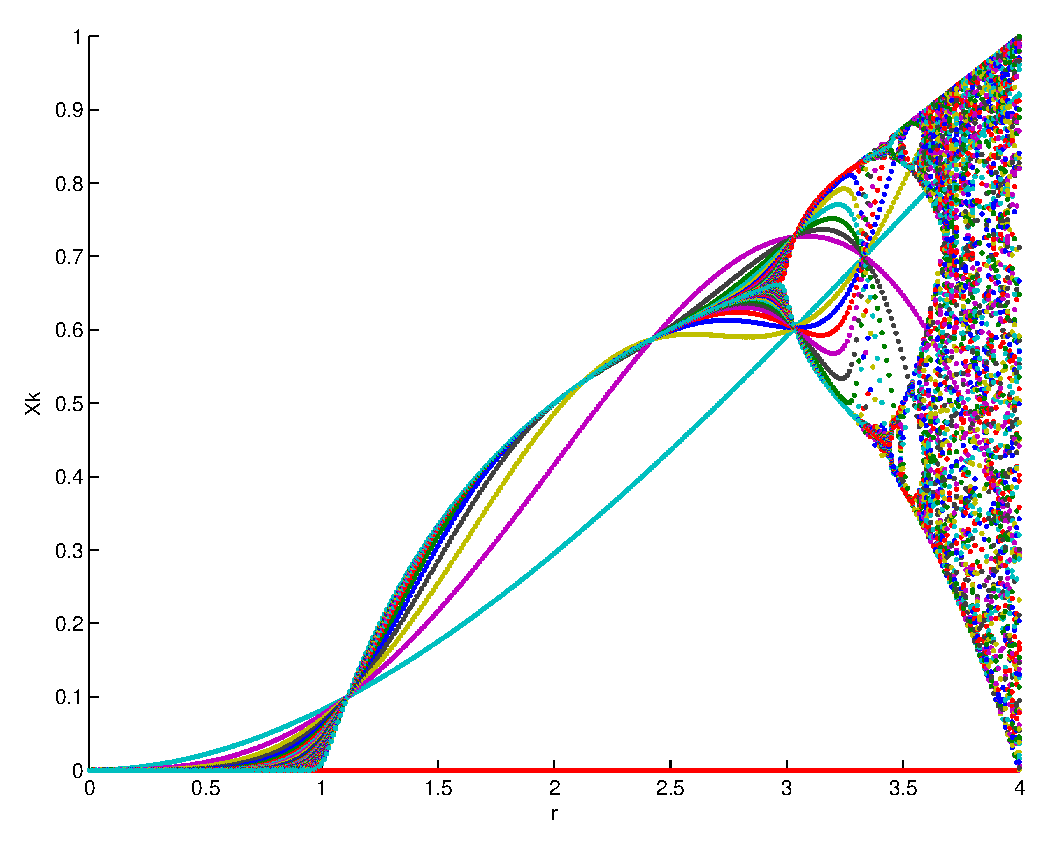
\includegraphics[scale=0.3]{EPSFiles/LogisticAllXk}

    \caption{Logistic map - plotting all iterations of $x_{k}$ against values of $r$ in range $0 \leq r < 4$.}

    \label{LogisticAllXk}

\end{figure}

The following figure shows the bifurcation diagram for the logistic map by only plotting the large values of $x_{k}$.

\begin{figure}[H]

    \centering

    \includegraphics[scale=0.3]{EPSFiles/LogisticDots}

    \caption{Logistic map with $x_{0} = 0.1$. $0 \leq r < 4$.}

    \label{LogisticDots}

\end{figure} 

Again, this is quite similar to the corresponding figure for the Verhulst map, with a few fairly
 obvious differences. %The general shape of the graph, with the period doubling cascade, is essentially the same as with the Verhulst map. 
  A key difference is that the single attractor doesn't have the same value for all $r \textrm{-values}$. The value of the attractor
     increases as $r$ increases, giving the bifurcation diagram a curved shape for $1 < r < 2$, rather
     than a straight line, like in the Verhulst map. For $r$ in the range $0 \leq r < 1$, the
       single attractor has a value of 0, because the equation is $x_{k + 1} = rx_{k}(1 - x_{k})$, and
        all terms in this product are between 0 and 1, so $x_{k}$ will always decrease. 
Another difference is that the logistic map is kind of, briefly ignoring
 the differences mentioned in the previous paragraph, translated by one unit to the right. 
 In particular, all period doubling points, and the point where it becomes chaotic, are one unit bigger in the logistic map.
Once the period doubling starts, these two maps look nearly identical. This is especially true
 once the chaotic section of the map starts, and there is even a three-cycle attractor appearing inside
  the chaotic section of the logistic map, which was apparent in the Verhulst map. 

\begin{figure}[H]

    \centering

    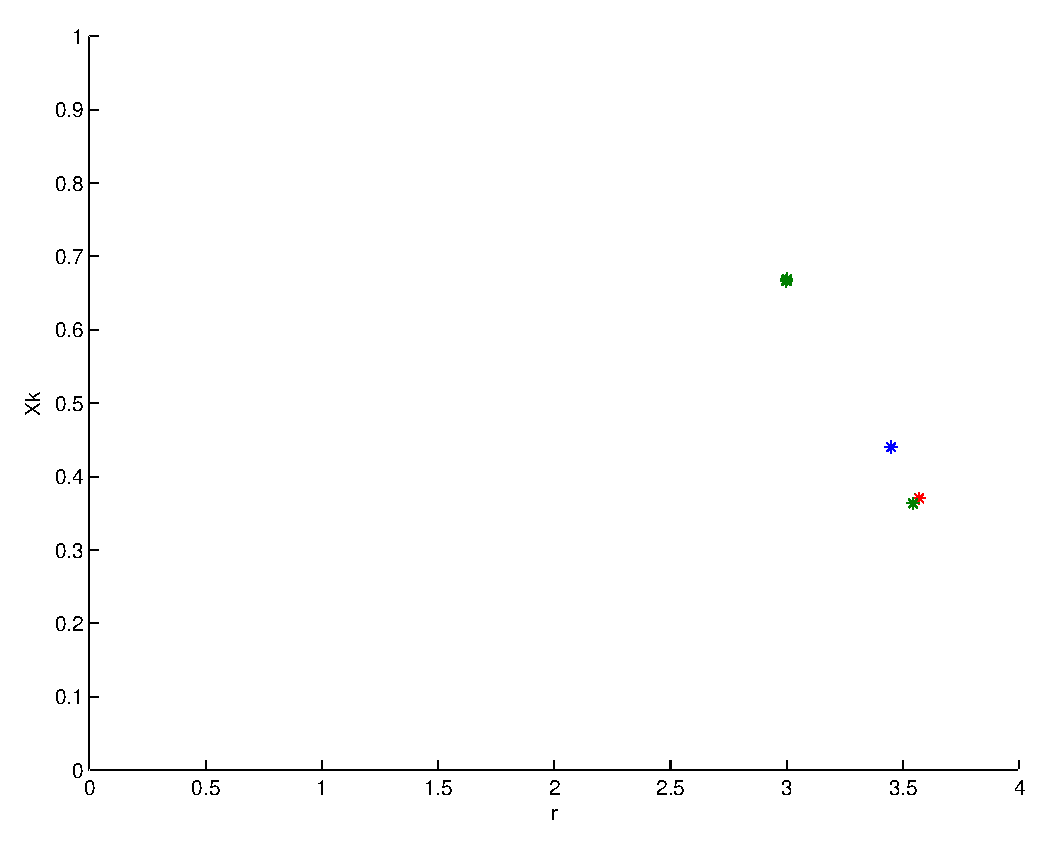
\includegraphics[scale=0.2]{EPSFiles/MAINLogisticPointsEPS}

    \caption{The $r \textrm{-values}$ on the logistic map, from the figure above, where period doubling
     occurs. These are exactly one more than the corresponding points on the Verhulst map.}

\end{figure} 

When the initial $x$ value is 0, the figure for the logistic map is just a straight horizontal line
 with value 1, because $x_{1} = rx_{0}(1 - x_{0})$, where $x_{0} = 0$, so $x_{1} = 0$. This pattern
  carries on, so $x_{k} = 0$ $\forall k \geq 0$. For $0 < x_{0} < 1$, the figure shows the same pattern
   as the $x_{0} = 0.1$ figure from earlier in this section, and, just like the Verhulst map, as $x_{0}$ changes in this range, some
    of the points change places, while keeping the same shape. $x_{0} = 1$ has exactly the same figure as $x_{0} = 0$, because now $(1 - x_{0}) = 0$, so all $x_{k} = 0$. When $x_{0} > 1$, only the part of the figure between $r = 0$ and $r = 1$ has any points
       plotted. As $x_{0}$ increases above 1, the smallest $r \textrm{-value}$ such that
         all larger values cause divergence, or zero attractors, decreases. Again, this is the same as
          in the Verhulst map, where the domain decreases more and more.

\begin{figure}[H]
        \centering
        \begin{subfigure}[b]{0.2\textwidth}
                \includegraphics[width=\textwidth]{EPSFiles/Logistic0}
                \caption{$x_{0} = 0$}
        \end{subfigure}
        \begin{subfigure}[b]{0.2\textwidth}
                \includegraphics[width=\textwidth]{EPSFiles/LogisticDots}
                \caption{$x_{0} = 0.1$}
        \end{subfigure}
        \begin{subfigure}[b]{0.2\textwidth}
                \includegraphics[width=\textwidth]{EPSFiles/Logistic09}
                \caption{$x_{0} = 0.9$}
        \end{subfigure}
        
        \begin{subfigure}[b]{0.2\textwidth}
                \includegraphics[width=\textwidth]{EPSFiles/Logistic1}
                \caption{$x_{0} = 1$}
        \end{subfigure}
        \begin{subfigure}[b]{0.2\textwidth}
                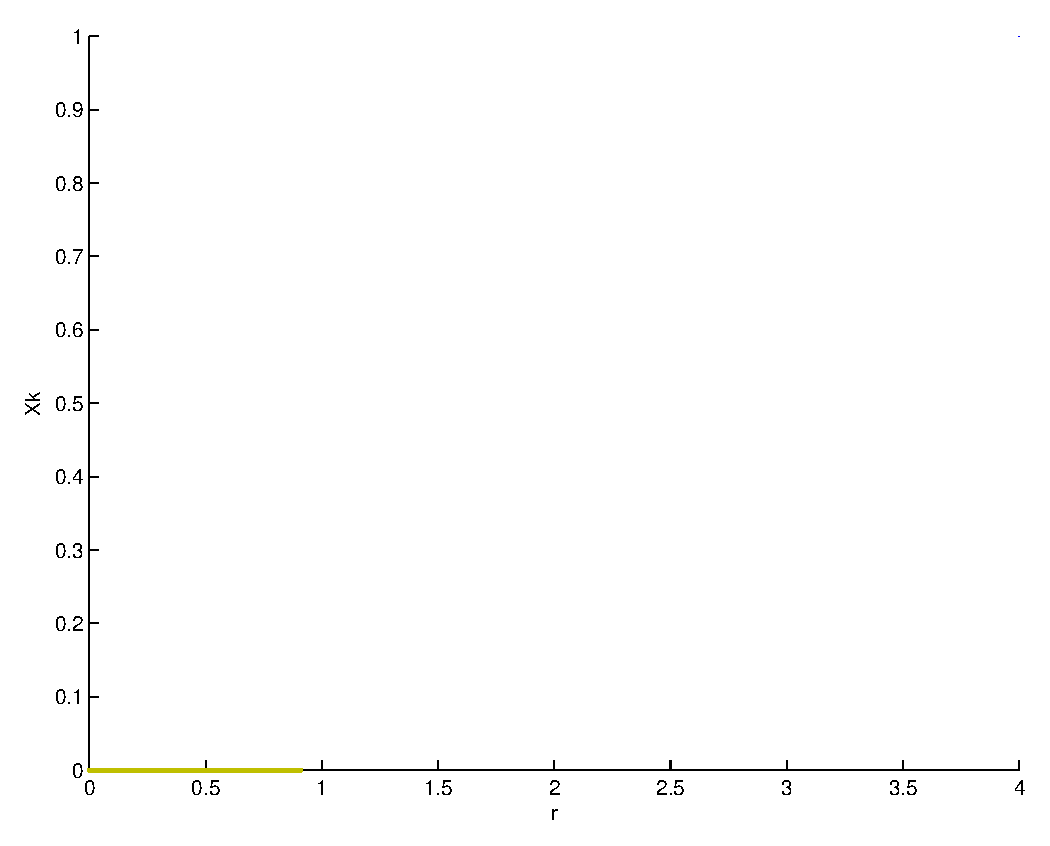
\includegraphics[width=\textwidth]{EPSFiles/Logistic11}
                \caption{$x_{0} = 1.1$}
        \end{subfigure}  
        \begin{subfigure}[b]{0.2\textwidth}
                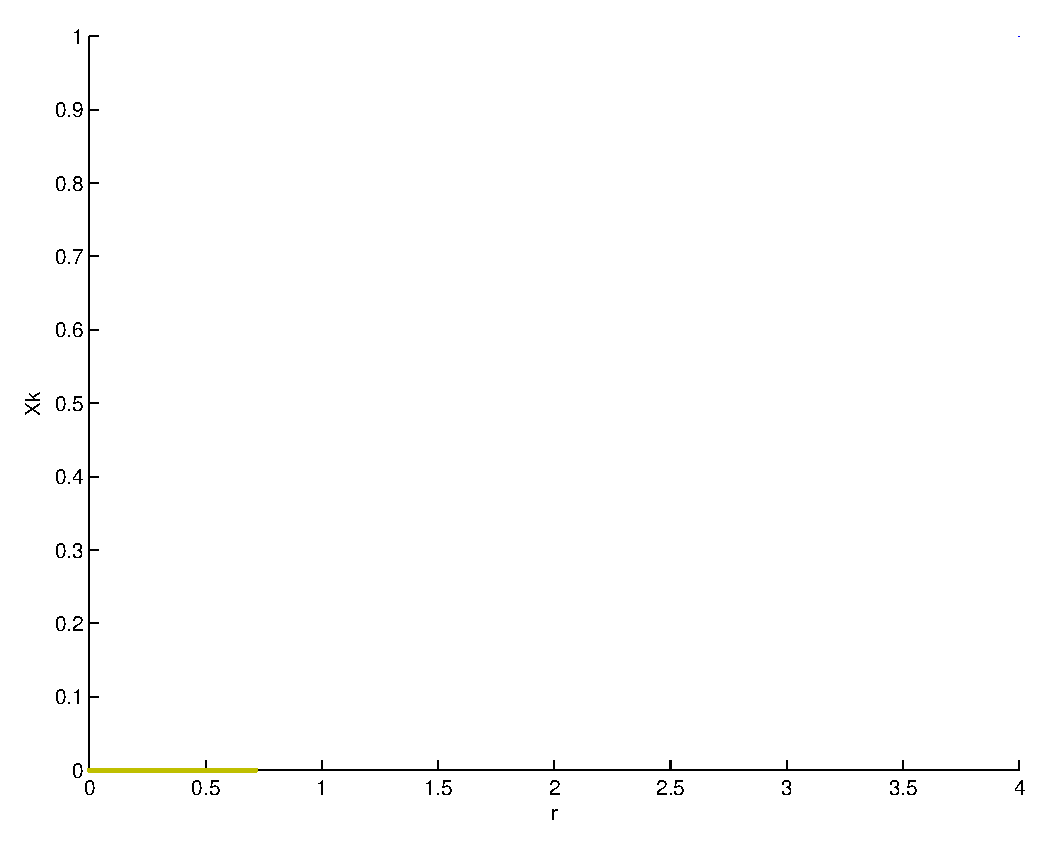
\includegraphics[width=\textwidth]{EPSFiles/Logistic14}
                \caption{$x_{0} = 1.4$}
        \end{subfigure}  
        \caption{Changing initial $x \textrm{-value}$ for Logistic map.}
\end{figure}

The fact that these two maps are so similar shouldn't really come as too much of a surprise, as their
 equations are so similar.

\subsection{Trigonometric Map}

The trigonometric map is another non-linear one-dimensional map, similar to the Verhulst and logistic
 maps. It is defined by: 

\[
  x_{k+1} = rsin(x_{k}) \textrm{, for \emph{k}} \geq 0
\]

%(MAYBE DIFFERENCES WITH INTERWEAVING LINES WITH FIGURE, although I don't think this should go in - not much to say and figure is unnecessary)

The main figure for the trigonometric map, obtained by only plotting the large values of $x_{k}$, is
 shown below.

\begin{figure}[H]

    \centering

    \includegraphics[scale=0.3]{EPSFiles/TrigonometricDots}

    \caption{Trigonometric map with $x_{0} = 0.1$. $0 \leq r < 3$. However, graph would carry on for $r \geq 3$.}

\end{figure} 

All 3 of these non-linear one-dimensional maps covered so far are very similar, as you can see from their bifurcation diagrams. 
 The trigonometric map, however, has
  some key differences. Most notably, although not shown in the above figure, there is no $r
   \textrm{-value}$ such that all larger values of $r$ cause divergence, or no attractors. The diagram
    will carry on having either  attractors or chaos for all $r \textrm{-values}$. This is most likely due to the periodic nature of the sine curve - the infinite repetition. 
          Another thing we can say about the figures is that the number of period doubles seems to
           become infinite at $e$ - the exponential constant, which seems rather strange. This will
            become slightly clearer in the next figure.

%Took out not figure with not just large Xk - interweaving lines : I MISS IT PLEASE PUT IN PRESENTATION :'(

\begin{figure}[H]

    \centering

    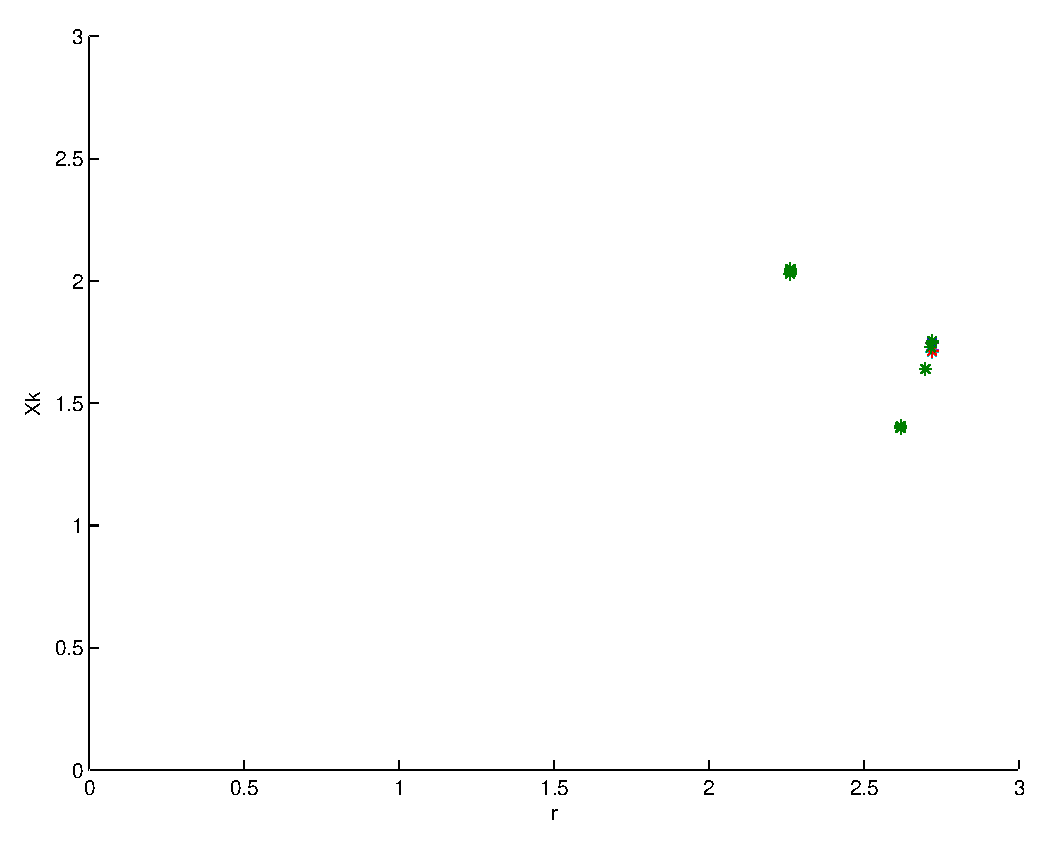
\includegraphics[scale=0.2]{EPSFiles/MAINTrigonometricPointsEPS}

    \caption{The $r \textrm{-values}$ on the trigonometric map, from the figure above, where period doubling occurs.}

\end{figure} 

From the above figure, we can see that the first $r \textrm{-values}$ where period doubling occurs are
 2.261, 2.6173, 2.6973, and 2.7146. It seems like these values are tending to $e$.

%BILLIANT - not a spelling mistake (Kiran)
The figures below show what the bifurcation diagram looks like when $x_{0}$ is varied. $x_{0} = 0$,
 $x_{0} = \pi$, and $x_{0} = 2\pi$ result in the figure being a straight line with the single attractor
  having a value of 0. This is because $sin(0) = 0$, $sin(\pi) = 0$, and $sin(2\pi) = 0$, and the
   differential equation defining this map is $x_{k+1} = rsin(x_{k})$, so clearly all $x_{k}$ will be
    0. For $0 < x_{0} < \pi$, the bifurcation diagram is 'positive', as seen in figures (b) and (c)
     below, and for $\pi < x_{0} < 2\pi$, it is negative, as seen in figures (d) and (e) below. This
      pattern repeats itself, so $\forall k \in \mathbb{Z}$, $x_{0} = k\pi$ results in the
       aforementioned straight line figure (see figure (a) below), $2k\pi < x_{0} < (2k + 1)\pi$
        results in a positive figure (see figures (b), (c) and (f) below), and $(2k + 1)\pi < x_{0} <
         (2k + 2)\pi$ results in a negative figure (see figures (d) and (e) below). This clearly
          happens because of the values that $sin(x_{k})$ will take with these $x_{0}$ values, and thus
           further $x_{k}$ values.

\begin{figure}[H]
        \centering
        \begin{subfigure}[b]{0.25\textwidth}
                \includegraphics[width=\textwidth]{EPSFiles/Trigonometric0}
                \caption{$x_{0} = 0$}
        \end{subfigure}
        \begin{subfigure}[b]{0.25\textwidth}
                \includegraphics[width=\textwidth]{EPSFiles/Trigonometric15}
                \caption{$x_{0} = 1.5$}
        \end{subfigure}
        \begin{subfigure}[b]{0.25\textwidth}
                \includegraphics[width=\textwidth]{EPSFiles/Trigonometric314}
                \caption{$x_{0} = 3.14$ (Just under $\pi$)}
        \end{subfigure}
        
        \begin{subfigure}[b]{0.25\textwidth}
                \includegraphics[width=\textwidth]{EPSFiles/Trigonometric315}
                \caption{$x_{0} = 3.15$ (Just over $\pi$)}
        \end{subfigure}
        \begin{subfigure}[b]{0.25\textwidth}
                \includegraphics[width=\textwidth]{EPSFiles/Trigonometric628}
                \caption{$x_{0} = 6.28$ (Just under $2 \pi$)}
        \end{subfigure}  
        \begin{subfigure}[b]{0.25\textwidth}
                \includegraphics[width=\textwidth]{EPSFiles/Trigonometric629}
                \caption{$x_{0} = 6.29$ (Just over $2 \pi$)}
        \end{subfigure}  
        \caption{Changing initial $x$ value for Trigonometric map.}
\end{figure}

As a side note, the Trigonometric and Logistic maps were both explored using the cobweb
 diagram initially, re-enforcing the points made above. Some diagrams of there are shown below:
 
\subsection{Fractal Properties}

The main properties that define a fractal are self-similarity and non-integer dimension\cite{Fractal Properties}. The self-similarity, on all scales, means that if you zoom in on particular parts of the fractal, the original image will be reproduced, which means that you can zoom in again on this new image and repeat the process forever. The non-integer dimension is harder to explain, but this condition basically means that simple zero-dimensional points, one-dimensional lines, or two-dimensional curves, etc. cannot be classed as a fractal. 

Consider the Verhulst map bifurcation diagram discussed earlier, and recall the 3-cycle that appears in the chaotic section at about r = 2.828. Zooming in on one of the middle branch of this 3-cycle produces the following figure: 

\begin{figure}[H]

    \centering

    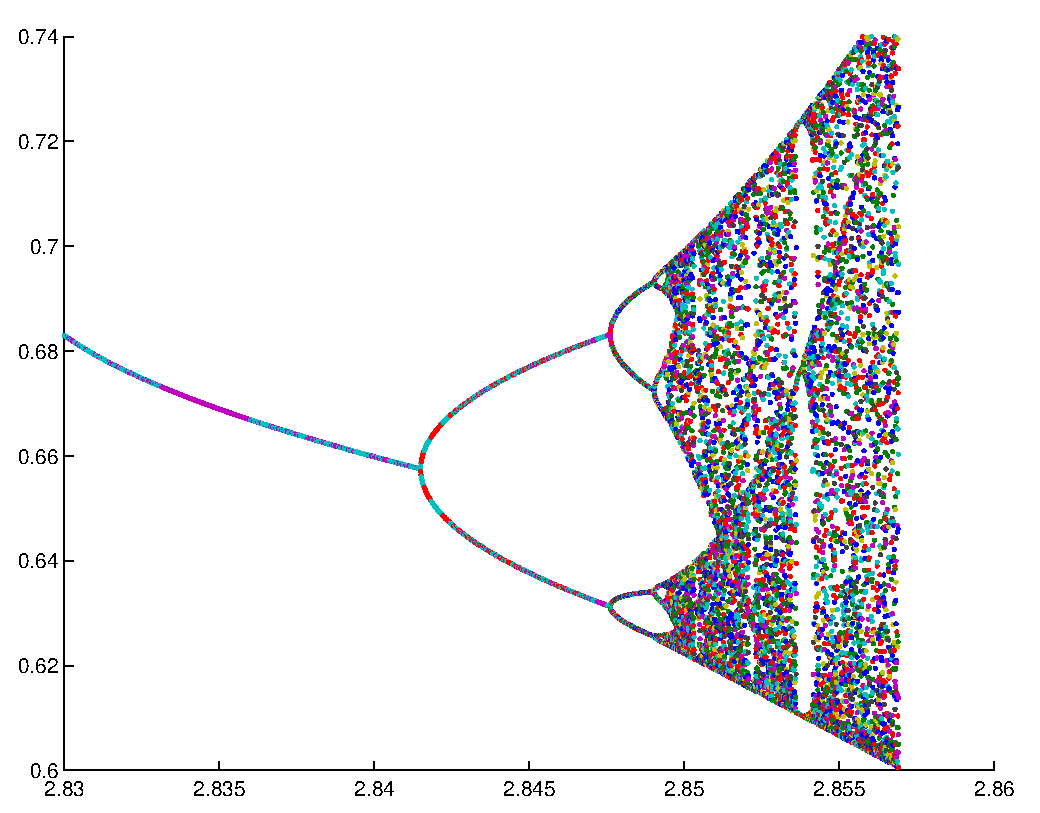
\includegraphics[scale=0.25]{EPSFiles/VerhulstFractal}

    \caption{Self-similarity of the Verhulst map.}

\end{figure} 

This is the same as the original bifurcation diagram, but on a different scale, which shows that the Verhulst map displays fractal properties. The other maps discussed earlier display the same behaviour.

%The ... map with equation $y = f(x)$ displays fractal properties, huzzah! %(hahahaha)

%DEFO _ KIRAN :)
%MIDDLE OF 3-CYCLE ATTRACTOR REPLICATES ENTIRE DIAGRAM - FRACTAL (Self-similar on all scales etc- look on wikipedia for what makes a fractal http://en.wikipedia.org/wiki/Fractal - ctrl+f "Straight line")

\section{Mandelbrot Set}

The history of the Mandelbrot set begins with Gaston Julia and Pierre Fatou. Between 1917-1920 Fatou introduced the Julia set at a similar time to Gaston Julia. The Julia set is the set of points $z$  for which a rational function $R(z)$ is infinitely applied but does not approach infinity, and the Fatou set is the complement of this set. The Mandelbrot set is the set obtained from the recurrence relation: $ z^2_{n+1} = z_{n} + c$ with $z_{0} = c$ and $c \in \mathbb{C}$. 
\\There is much controversy surrounding the history of the Mandelbrot set. Two mathematicians Robert W. Brooks and Peter Matelski wrote and circulated a paper in 1978 containing the equation $ z^2_{n+1} = z_{n} + c$ and a crude image of the Mandelbrot set. 

However, as they only published the paper in 1981, a year after Mandelbrot wrote his first article on
 the subject, they have received little recognition. In addition, John H. Hubbard had found a way to
  plot the output of iterative functions which he showed to Mandelbrot in the IBM's Thomas J. Watson
   research centre. This is where Mandelbrot would later develop another way to produce the Mandelbrot
    set in 1980. In spite of this controversy, Mandelbrot did important research on fractals including showing their importance in nature. An article in 1985 in the
      Scientific American helped popularise the Mandelbrot set to a wider audience. Today the idea of
       fractals and the Mandelbrot set has become so ingrained in popular culture that there are many
        phone apps such as 'Fractoid' dedicated to producing images of fractals. 
   
\subsection{Mandelbrot Set Itself}

\begin{figure}[H]
\centering
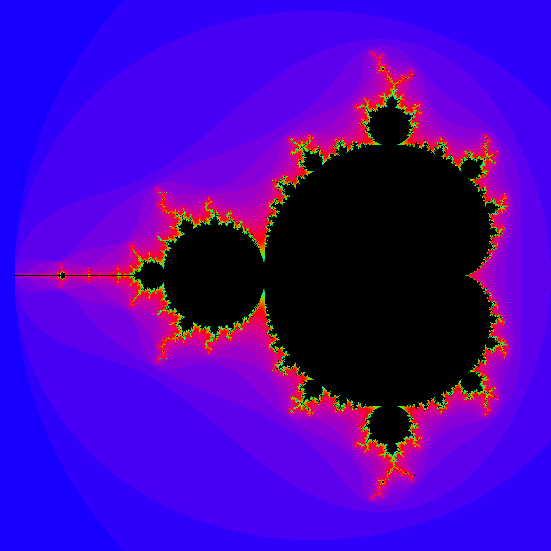
\includegraphics[scale=0.4]{MandelbrotSet/mandelbrot.png}
\caption{Mandelbrot Set}
\end{figure}

The image above of the Mandelbrot set shows the location of the c values in a complex
   plane which remain bounded, coloured in black. The furthest c value from the origin in the set is the complex number
    $-2+0i$. 
    
The image above was produced in Java using the build in BufferedImage Class. Each pixel in the image
 has been passed into the formula $z_{k+1} = z_{k}^{2} + c$ and repeatedly iterated at most 50 times,
  checking each time whether the modulus of the result is less than 2 (meaning is still bounded).
  
The different colours in the image of the Mandelbrot set above represent the number of iterations that
 were required until that particular pixel's orbit became unbounded (where the  $|z_{k}| > 2$).
  Creating a colour map in Java seemed relatively difficult and therefore as the figure below shows, a
   combination of cosine and sine representing the intensities of red,green and blue were used to colour the pixels according to how often they iterated.
    Any pixel where $|z_{k}| <= 2$ after 50 iterations  was coloured black. 
\begin{figure}[H]
\centering
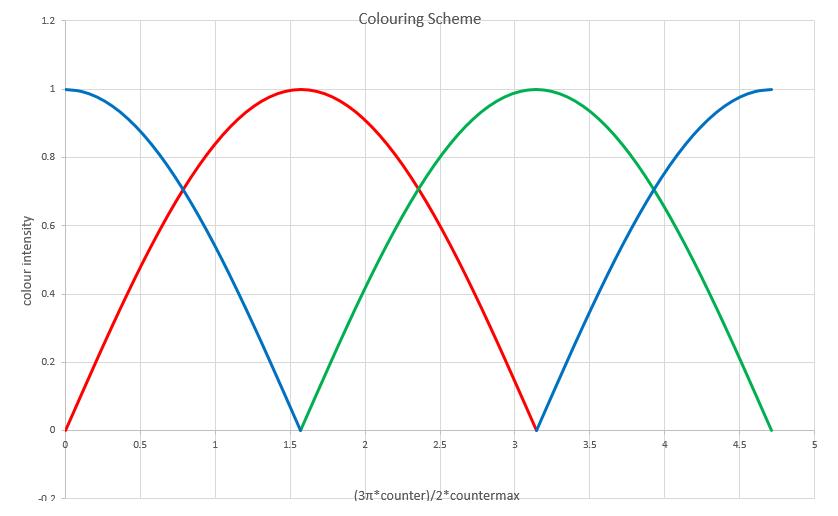
\includegraphics[scale=0.3]{MandelbrotSet/colourscheme.png}
\caption{Graph for colouring scheme of Mandelbrot set in figure above.}
\end{figure}
Further observations have shown that the higher the number of iterations for a given c before $|z_{k}|
 > 2$, the closer that particular c is to the edge of the Mandelbrot set - the fringe. Moreover these c
  values on the fringe may not necessarily reside in the set if the number of iterations is increase as
   less of them make it through the full amount of iterations satisfying the condition $|z_{k}| <= 2$.
    Therefore the fringe gets more detailed with  greater number of iterations and also by reducing the
     gap between the c values or increasing the number of c values tested (larger image produced).
      However increasing the number of iterations and number of c values rapidly decreased the overall
       performance of our code as there are more iterations to be performed overall resulting in longer
        runtime.

Above we mentioned that in order for a c value to be bounded, the $|z_{k}| <=2$ The proof for this is shown below:

Let $z_{1}$ = c, $z_{2}$ = $c^2 +c$...\\
If at any point in the iterative process the two conditions hold that $|z_{k}|$ is bigger than both $|c|$ and 2 then it can be shown that $|z_{k+1}| >|z_{k}|$ and so with further iteration the sequence would continue to grow to $\infty$.
\begin{align*}
        \mathbf{\frac{|(z_{k+1})|}{|z_{k}|}} &= \mathbf{\frac{|z_{k}^2 + c|}{|z_{k}|} } 
        \\
        & \mathbf{\geq \frac{|z_{k}|^2-|c|}{|z_{k}|}} \qquad [triangle\ inequality ]  \\ 
        &= \mathbf{|z_{k}| - \frac{|c|}{|z_{k}|} } \\
        &> \mathbf{|z_{k}| -1}   \qquad\hspace{0.45cm}[ |z_{k}| > |c| ] \\ 
        &> \mathbf{1} \qquad \hspace{1.42cm} [ |z_{k}| > 2 ]
\end{align*}
Therefore $|z_{k+1}| > |z_{k}|$ and so the sequence is unbounded. \\   \\
However whilst writing the iterative loop to create the Mandelbrot set, our variant was just: $|z_{k}| <=2$ or $counter < countermax$. There was no checking of $|z_{k}| <= |c|$. The reason  is if $|z_{k}| >2$ then $|z_{k}| > c $ which is shown below.
Assuming $|z_{k}| >2$, there are 2 possibilities:
\begin{list}{*}{}
\item If $|c| >2$ then $|c^2+c| \geq |c|^2 -|c| = |c|(|c|-1) > |c| $ for all $k >= 2$ so the iteration would stop.
\item If $|c| \leq 2$ then obviously $|z_{k}| > c $ for all k and again iteration stops.
\end{list}

Compact set:

%How compact sets are defined depends on how general the topological space is. A topological space is a
% set of points, where each point has a set of neighbourhoods.

%A neighbourhood of a point is a set which contains both that point and all the positions that point is allowed to move to. If we let X be a set %and have a function N assigning to each x in
%  the set X a collection of subsets of X then the elements of N(x) are neighbourhoods of x. The
%   function N must follow the axioms below for “X with N” to be a topological space.

%1)Each point belongs to every one of its neighbourhoods

%2)Every superset of a neighbourhood of a point is a neighbourhood of the point.

%3)The intersection of two neighbourhoods of a point is a neighbourhood of that point

%4)Any neighbourhood N of x contains a neighbourhood M of x such that N is a neighbourhood of each point
 %of M.

%Now that we know these definitions, we are able to define a compact set. 

Over any topological space, a compact set X occurs if there exists finite 
families of open sets that "cover" X and each point in X lies in some set within a family. 

%The meaning for open sets from the definition can be further expressed in a nice way in terms of neighbourhoods. 
%If U is open and defined to be a subset of a topological space then U must be a neighbourhood of all points in U. 

However, for a Euclidean Space the compactness of a set is equivalent to a set being closed and bounded. \cite{compactness} As we are considering the Mandelbrot set on the Cartesian plane this definition will suffice for our proof.\\
\emph{Proof that the Mandelbrot Set is a comapct set} \cite{compact proof}
\\Definitions:
\\$P_{c}(z) = z^2 + c$ and $Q_{n}(c) = P^n_{c}(0)$ where by $P^n$ we mean the 'nth' iteration of P.\\
\begin{wrapfigure}{r}{0.25\textwidth}
  \begin{center}
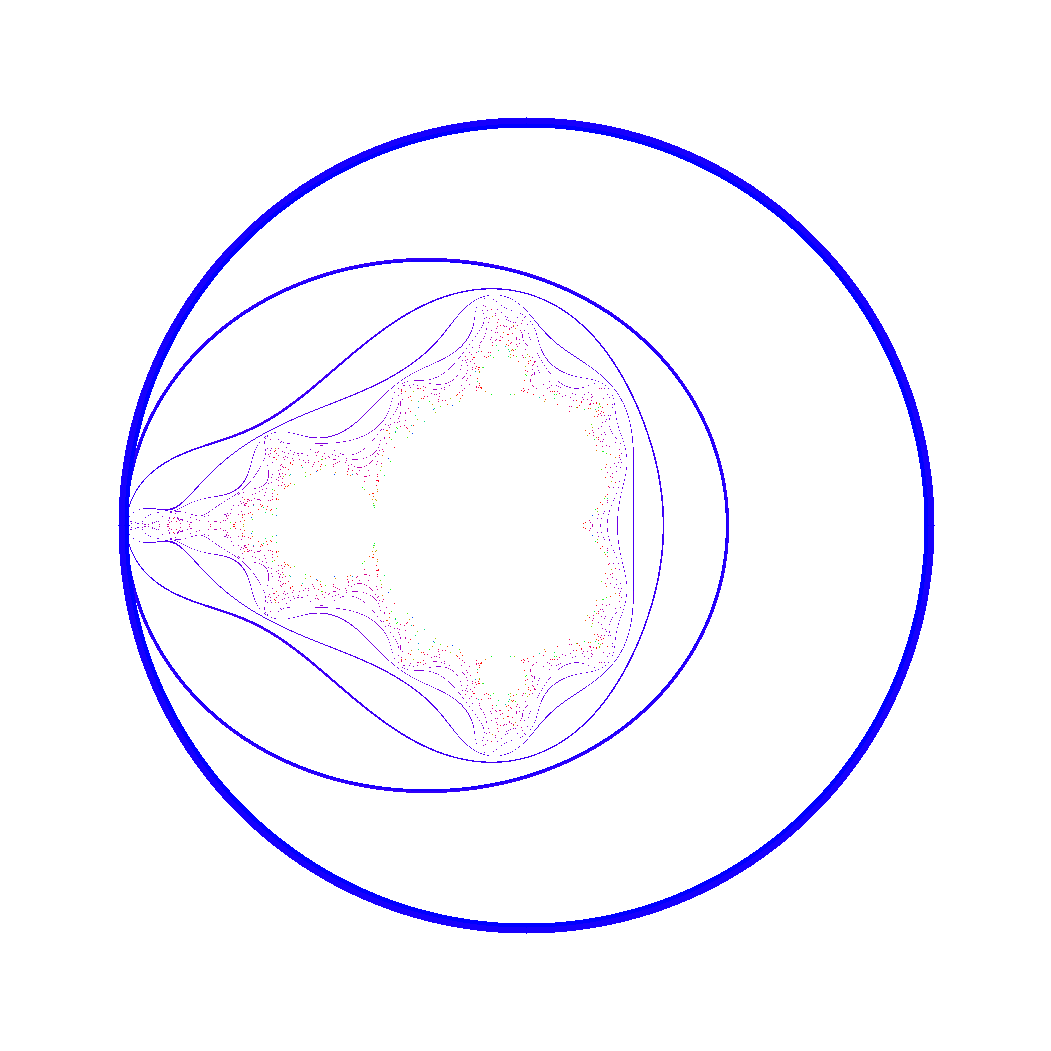
\includegraphics[width = 0.25\textwidth]{Compact/compact.png}
\vspace{-40pt}
\end{center}
\end{wrapfigure}
\\Our earlier proof showed that the Mandelbrot Set (denoted here as M) is contained in a closed disk of radius 2, therefore we can define M as: 
M =  $ \{ c \in \mathbb{C}; |Q_{n}(c)| \leq 2,  \forall n \in \mathbb{N}  \} $
\\Which can be expressed as:
\\ M = $\bigcap _{n=1}^\infty Q_{n}^-1(K)$ where $K = \{ z \in \mathbb{C}; |z| \leq 2 \}$
As $Q_{n}^-1(K)$ is closed and bouded for all n, M is the intersection of a compact set. This means that M is a compact set in $\mathbb{C}$.
\\The image to the right shows the progressive boundaries of the intersection $\bigcap _{n=1}^\infty Q_{n}^-1(K)$, which for large $n$ starts to form the outline of the Mandelbrot set. 

\subsection{Julia Sets}

%\emph{SOME HISTORY OF JULIA GUY}

The Julia Set for a rational function $R(z)$ where $z \in \mathbb{C}$  is defined as the set of points $z$ which do not approach infinity after $R(z)$ is repeatedly applied. \cite{Julia definition}
\\Quadratic Julia sets are generated using the quadratic maping $z_{k+1} = z_{k}^{2} + c$ for a fixed c, where $z \in \mathbb{C}$. Repeated iteration is carried out on each value of z checking
    whether it remains bounded ($z \leq 2$) . All values that are unbounded are
     then part of the Fatou set(the complement of the Julia Set).
   
    
The key link between the Mandelbrot set and the Julia Set is that a c value is in the
 Mandelbrot set if it's corresponding Julia set is connected. The meaning of
  connected is that one can trace a path from one point in the set to another point
   in the set without leaving the set. 

%For example as shown in the first figure below where we take c to be equal to 0, the
% Julia set formed is the unit circle. Two
 %  Fatou domains also exist: the interior and the exterior of the circle which iterate towards
 %   0 and $\infty$ respectively. The iteration process of the complex number on the border of this circle just doubles the angle. 

\begin{figure}[H]
        \centering
        \begin{subfigure}[b]{0.23\textwidth}
                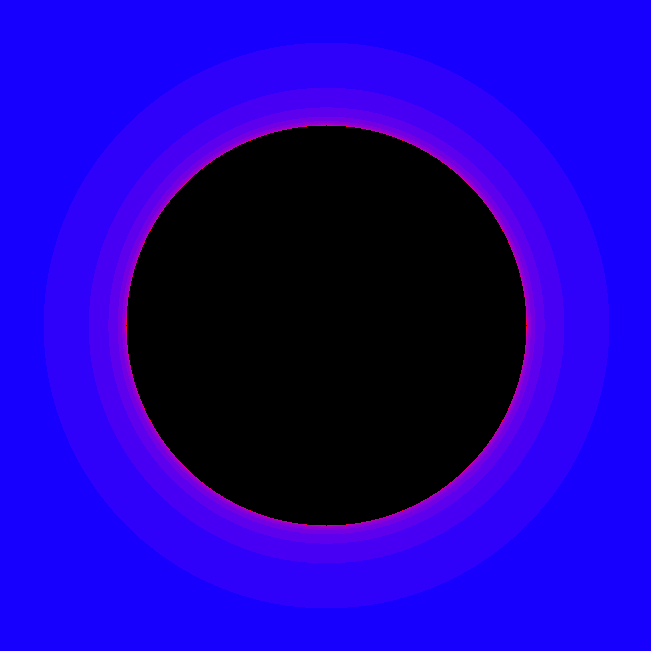
\includegraphics[width=\textwidth]{JuliaSets/julia1.png}
                \caption{c = $0$}
                \label{fig:c=0}
        \end{subfigure}
        \begin{subfigure}[b]{0.23\textwidth}
                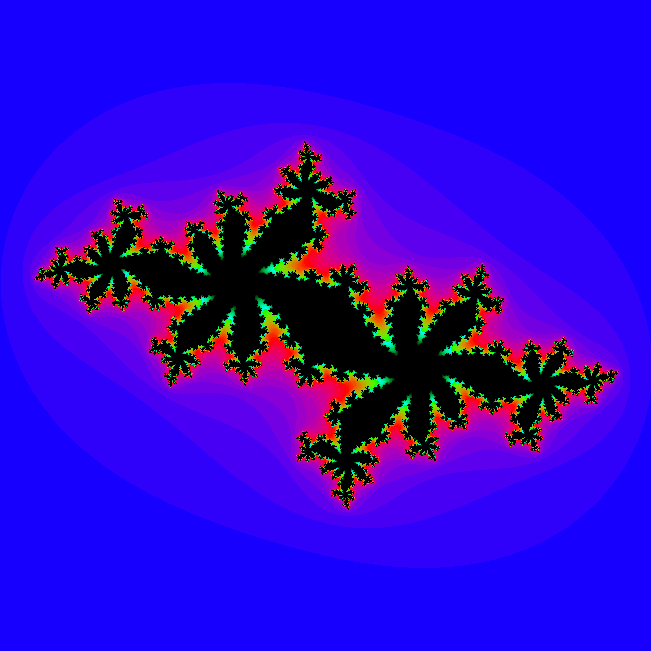
\includegraphics[width=\textwidth]{JuliaSets/julia2.png}
                \caption{c = $-0.624+0.435i$}
                \label{fig:c=-0.624+0.435i}
        \end{subfigure}       
        \begin{subfigure}[b]{0.23\textwidth}
                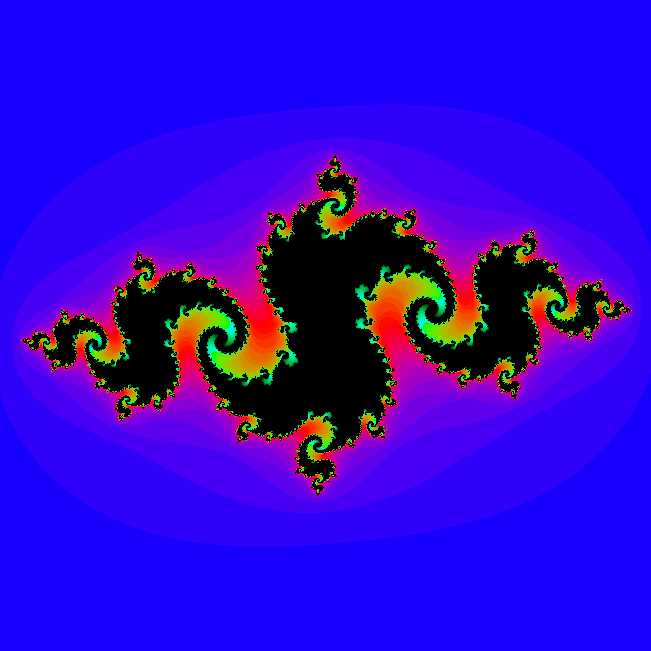
\includegraphics[width=\textwidth]{JuliaSets/julia3.png}
                \caption{c = $-0.8-0.15i$}
                \label{fig:c=-0.8-0.15i}
        \end{subfigure}        
        \begin{subfigure}[b]{0.23\textwidth}
                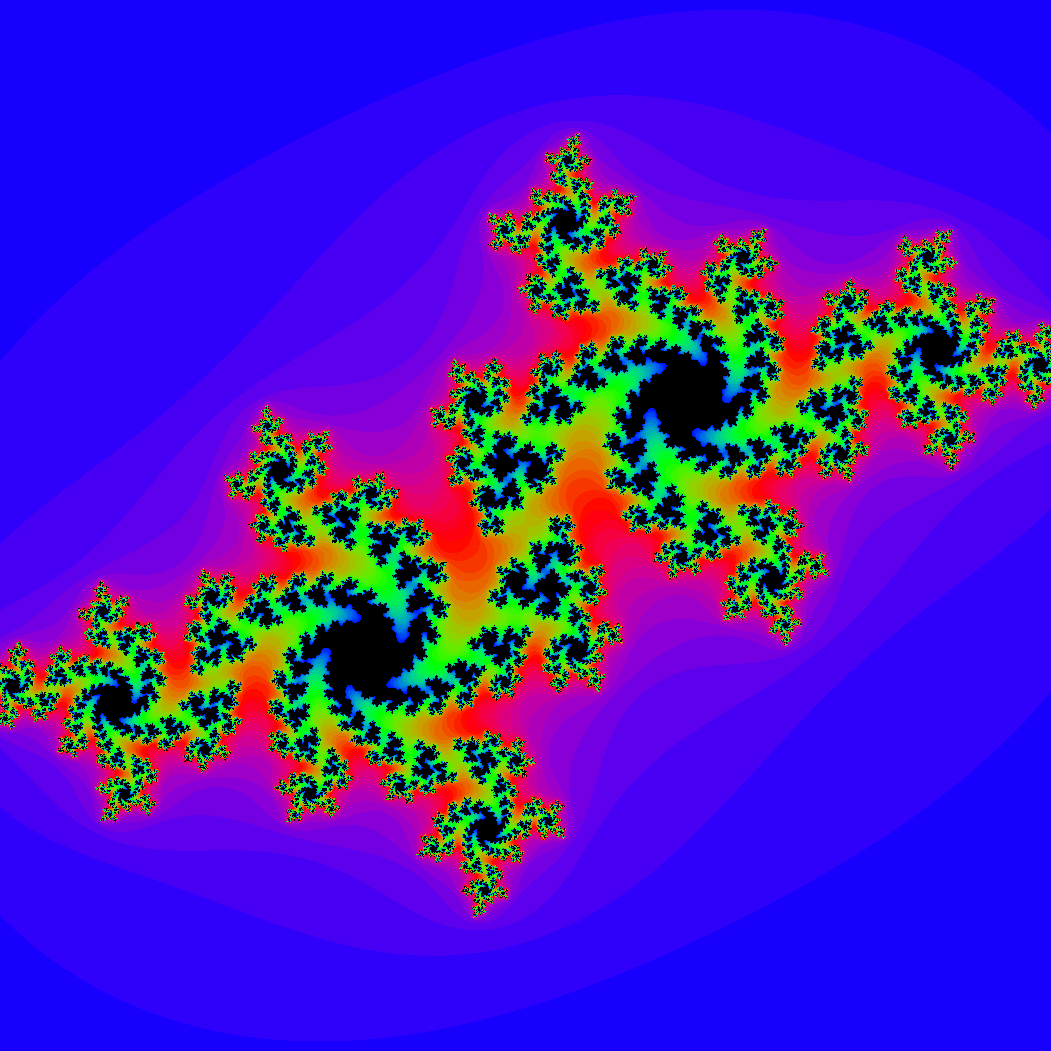
\includegraphics[width=\textwidth]{JuliaSets/julia4.png}
                \caption{c = $-0.46-0.59i$}
                \label{fig:c=-0.46-0.59i}
        \end{subfigure}
        \caption{Interesting images can be produced.}
\end{figure}

An interesting property we found was that the look of the Julia sets corresponds roughly to the look of
 the Mandelbrot set in a given region of c values. This depicts the fact stated before that the
  Mandelbrot Set is a map between all Julia sets in Space. The pictures below show a zoomed in region of the Mandelbrot set, you can make out some Julia sets that look like figure~\ref{fig:c=-0.46-0.59i}. The fractal property of the Mandelbrot set is also shown in these images as well, just as in the Verhulst process:  
   
\begin{figure}[H]
        \centering
        \begin{subfigure}[b]{0.24\textwidth}
                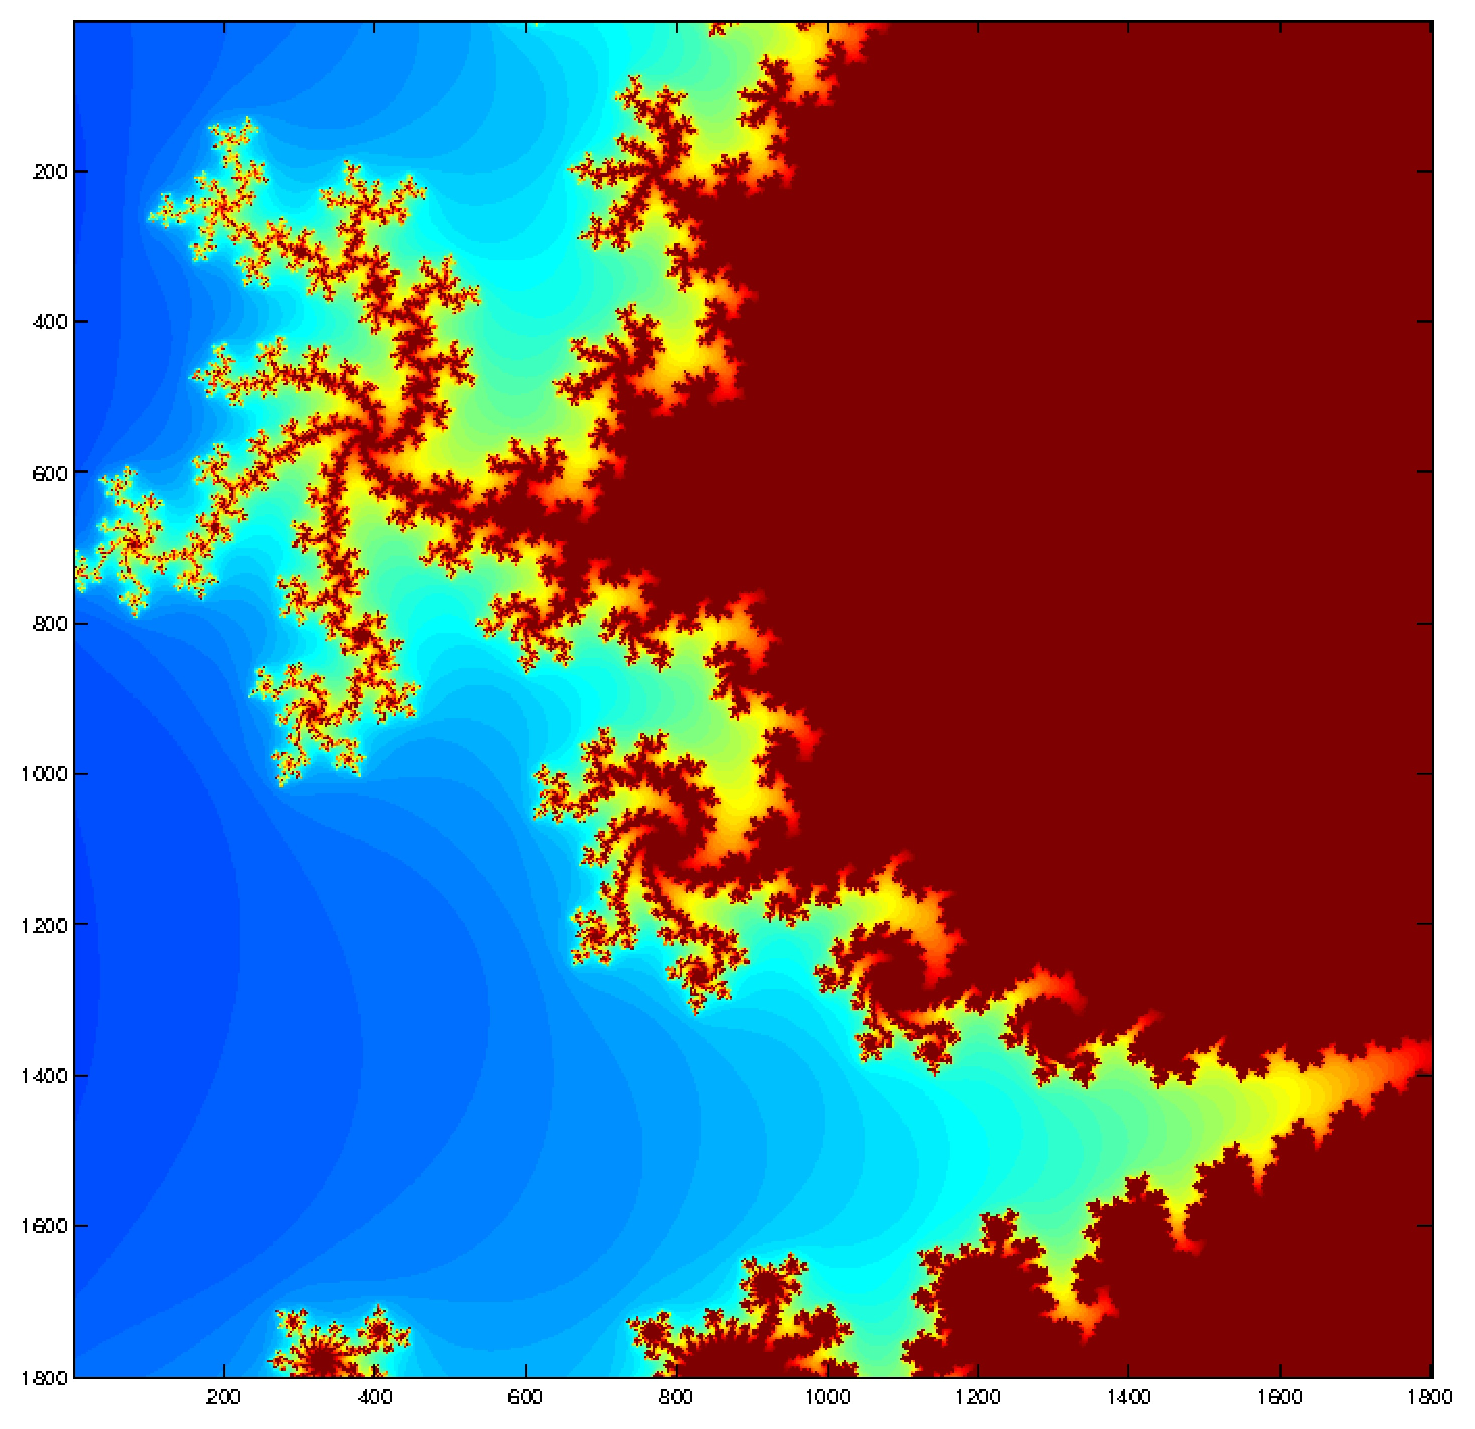
\includegraphics[width=\textwidth]{EPSFiles/MandelbrotZoom1}
                \label{fig:Zoom1}
        \end{subfigure}
        \begin{subfigure}[b]{0.24\textwidth}
                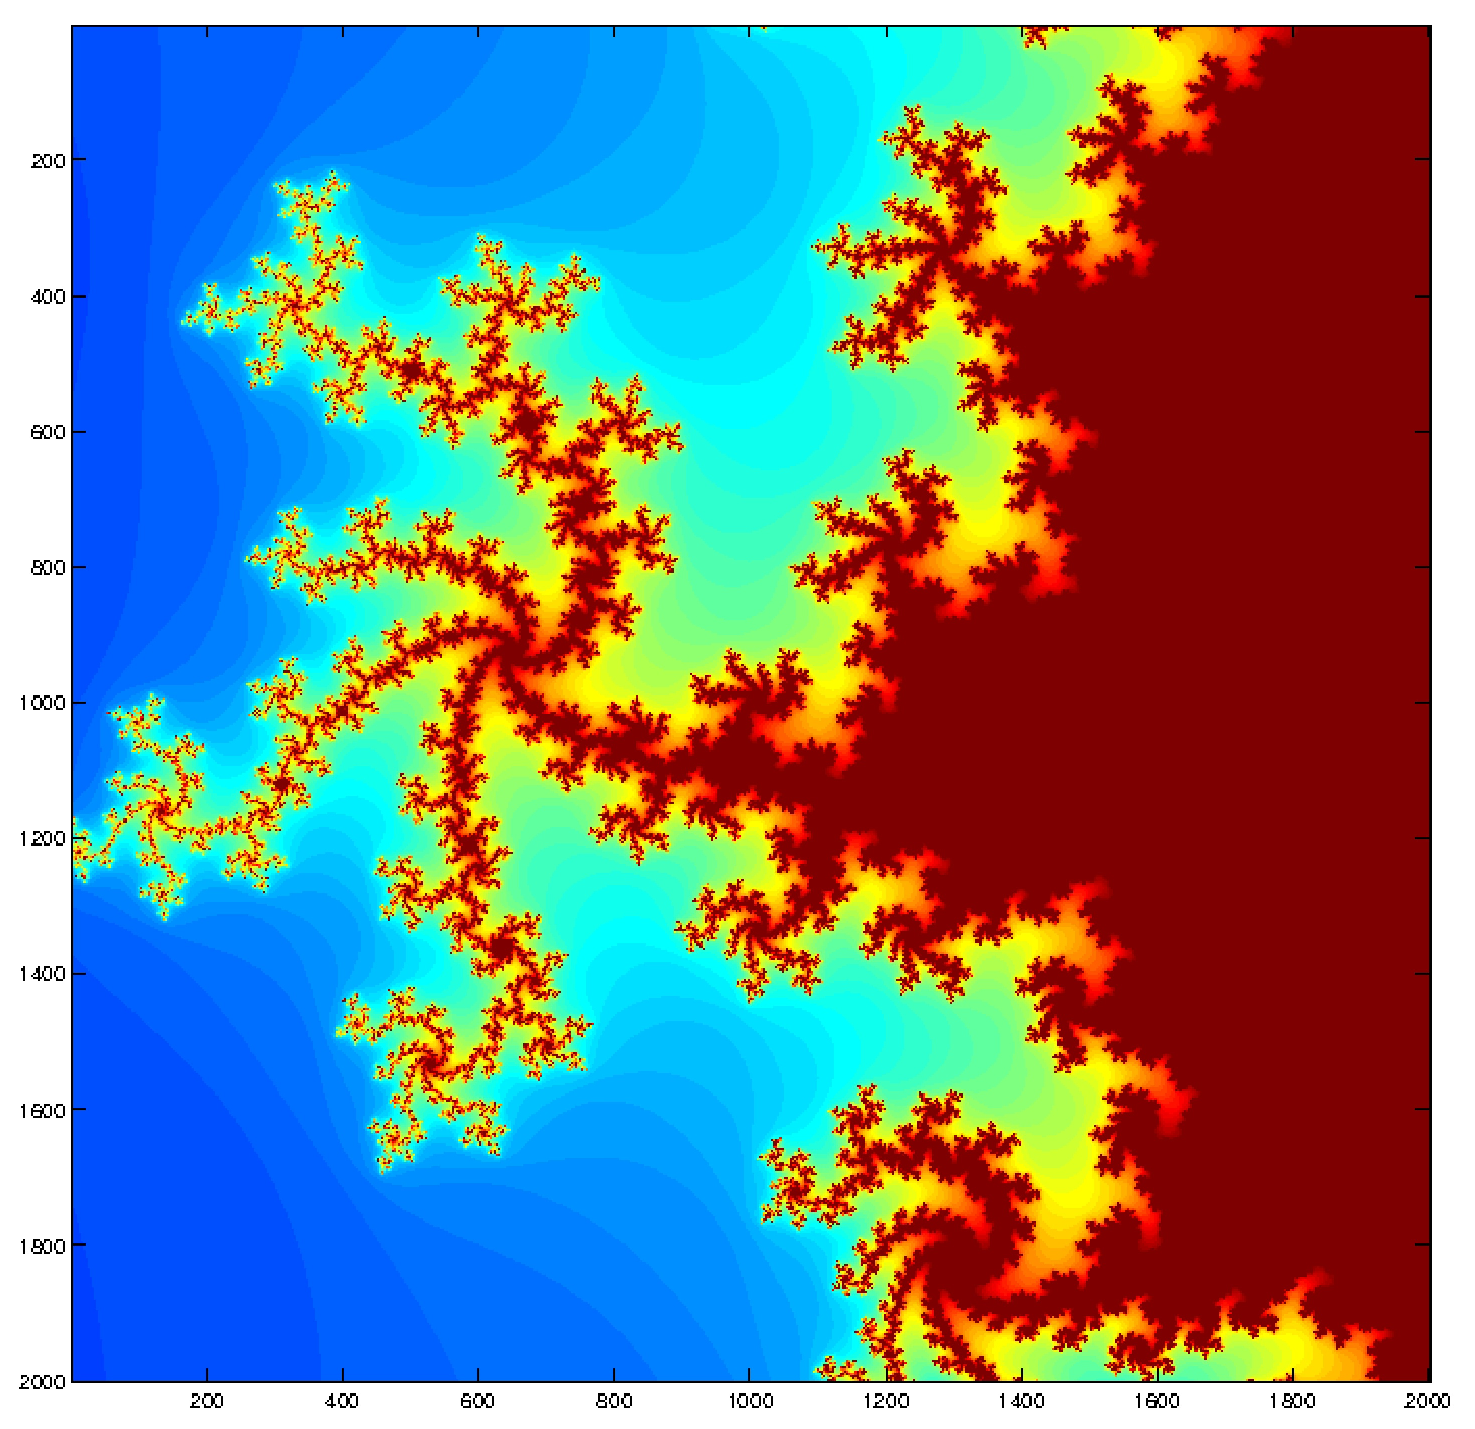
\includegraphics[width=\textwidth]{EPSFiles/MandelbrotZoom2}
                \label{fig:Zoom2}
        \end{subfigure}       
        \begin{subfigure}[b]{0.24\textwidth}
                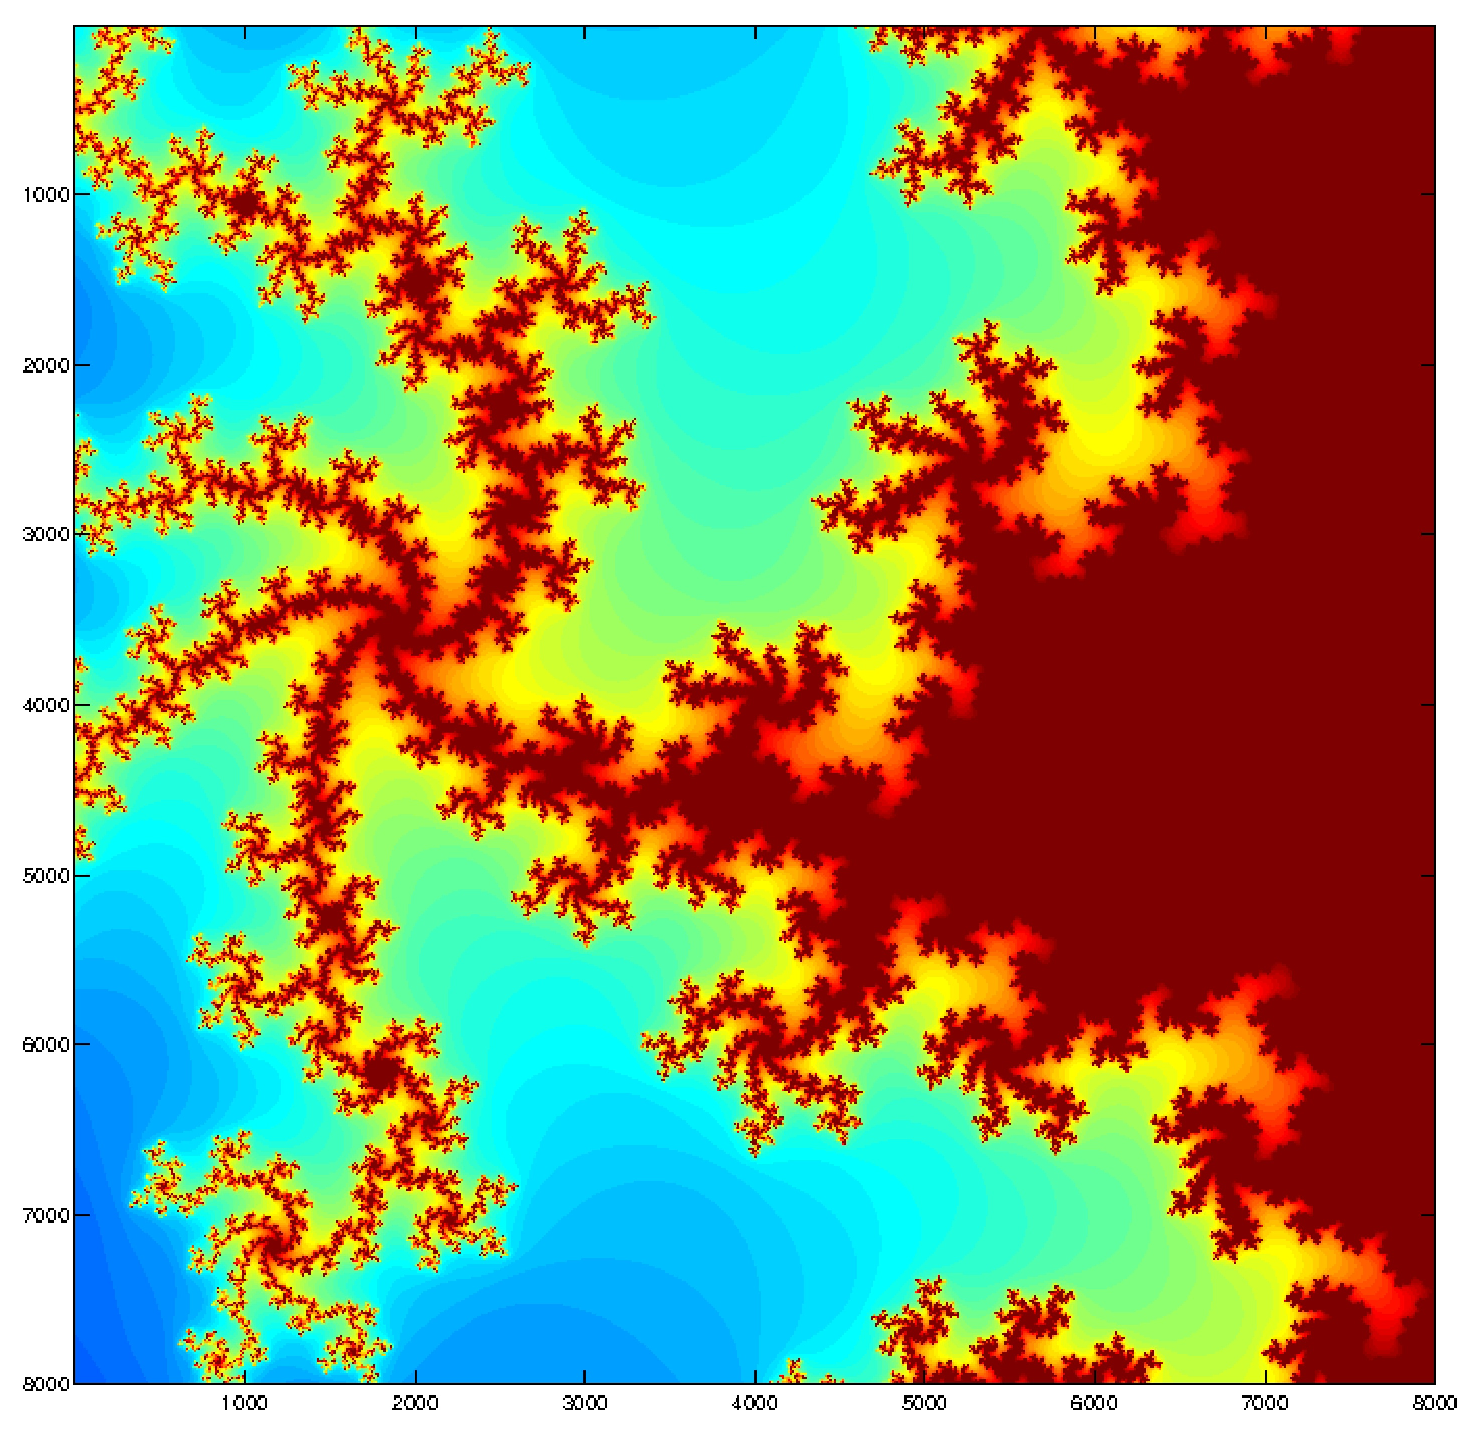
\includegraphics[width=\textwidth]{EPSFiles/MandelbrotZoom3}
                \label{fig:Zoom3}
        \end{subfigure}        
        \caption{Julia sets on the edge of the Mandelbrot Set}
\end{figure}

\subsection{Both Graphs - Bifurcation in Mandelbrot}
By investigating both the Mandelbrot set and the Verhulst Process
 it is quite interesting to see that they are both actually
  examples of a similar process. The Verhulst Logistic equation
   can undergo a sequence of linear transformations to obtain the
    same appearance as Mandelbrot's equation:

If we start with,
  \begin{center}
  $vk : x = kx(1-x)$
  \end{center}
and we take the equation,
  \begin{center}
  $ \Phi : x = \frac{1}{2} + \frac{x}{k} $
  \end{center}
then by doing the composition, 
  \begin{center}
  $ \Phi^{-1 }\circ vk \circ \Phi $
  \end{center}
we are get the following result,
  \begin{center}
  $ x = x^2 + (\frac{k}{2} - \frac{k^2}{4}) $
  \end{center}
  
As you can see this is similar to the Mandelbrot equation with
 the relationship $1-4c = (k-1)^2$\cite{Bifurcation in Mandelbrot Set 2}, this is only true along the
  real axis of the Mandelbrot set, meaning these real values
   correspond to different parts of the logistic map. In the figure 
    on the left below you can see the different $c \textrm{-values}$
     on the real axis of the set which correspond to the points of
      bifurcation talked about before in our analysis of the Verhulst
       process. 
   
   \begin{figure}[H]
        \centering
        \begin{subfigure}[b]{0.3\textwidth}
                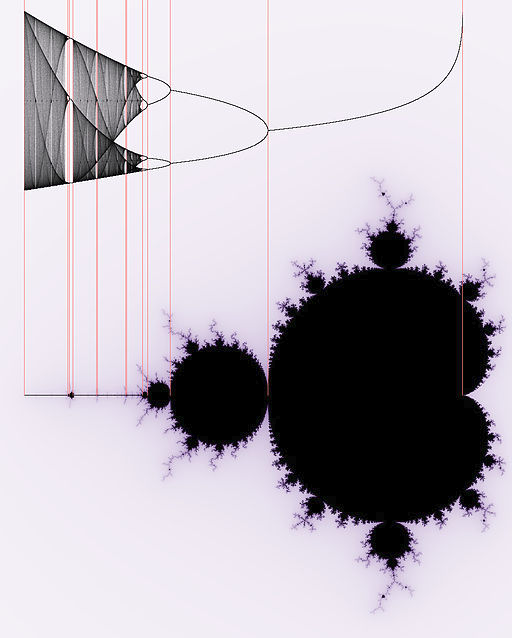
\includegraphics[width=\textwidth]{MandelbrotSet/Verhulst-Mandelbrot-Bifurcation}
                \caption{Real values of z linking to logistic map\cite{Bifurcation in Mandelbrot Set 1}}
        \end{subfigure}
        \begin{subfigure}[b]{0.3\textwidth}
                \includegraphics[width=\textwidth]{MandelbrotSet/Mandelbrot_Set_–_Periodicities_coloured}
                \caption{$x_{0} = 1.5$\cite{Bifurcation in Mandelbrot Set 2}}
        \end{subfigure}

        \caption{Linking the Mandelbrot set to the Verhulst Process}
\end{figure}

Cycles occur in the Mandelbrot set on different disks for a different starting $c \textrm{-value}$ .In
 the image on the right above, the large main disc holds all the $c-\textrm{values}$ that forms an
  iterative process with one attractor and the next disc to the left of the first one holds all $c-
  \textrm{values}$ for two attractors, this pattern of period doubling carries on as you move left
   through the center discs in the Mandelbrot set along the real axis. This also surprisingly similar
    to bifurcation in the Verhulst process. Some other $c \textrm{-values}$ in discs on the edges of
     the Main bulbs of the set give processes with different numbers of attractors such as a 5 or 7
      attracting cycle.  A subsection on Bolls Results underneath looks closely at what is happening at
       points where these regions in the image above meet.

\subsection{Boll's Results}

In 1991 the computer science graduate David Boll was investigating the Mandelbrot set. He was trying to
 show that only the point (-0.75,0) connected the cardioid with the disk to its left.
To show this he found the number of iterations until escape (here written as $n_{c}$) for (-0.75, $\epsilon$) based on the value of $\epsilon$. What
 he found were the relationships:\\
 
for $c = -0.75 + \epsilon i$ that $\epsilon n_{c} \to \pi$ as $\epsilon \to 0 $
\\for $c = 0.25$ + $\epsilon$ that $ \sqrt{\epsilon}n_{c} \to \pi$ as $\epsilon \to 0 $\\
 \\A Java program was created using JTable to repeat these results:
\begin{figure}[H]
\centering
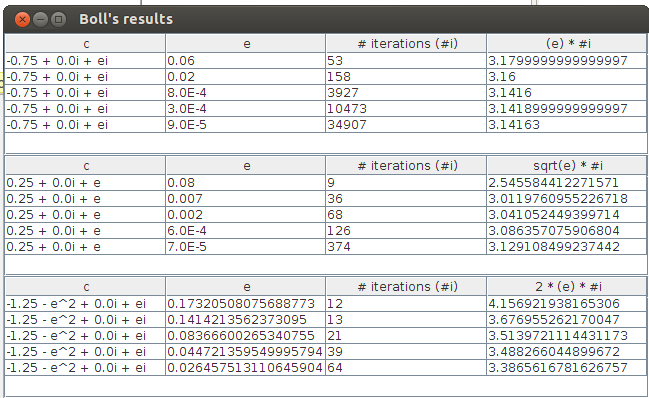
\includegraphics[scale=0.6]{BollsResults/finalboll.png}
\caption{Data for Boll's results.}
\end{figure}
In addition, in 1997 Jay Hill found that:
\\if $c= -1.25 - {\epsilon}^2 - \epsilon i$ then $\epsilon n_{c}\to \pi$ as $ \epsilon \to 0$\cite{Jay Hill}  \\
Which has been confirmed in the table above.
\\ \\These points have interesting geometric locations:
\begin{figure}[H]
\centering
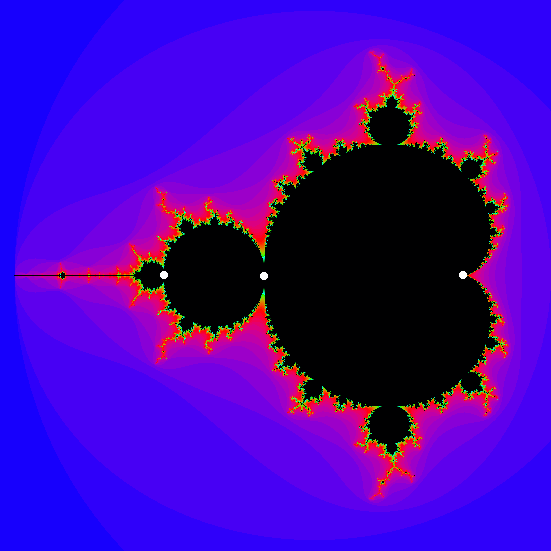
\includegraphics[scale=0.4]{MandelbrotSet/mandelbrotdot.png}
\caption{These positions from left to right are: (-1.25,0), (-0.75,0) and (0.25,0)}
\end{figure}
The positions (-1.25,0) and (-0.75,0) are interesting because they link the three largest disks on the real axis, and (0.25,0) is the largest point on the real axis which does not tend towards infinity.
\\It is clear that due to symmetry $c = -1.25 - \epsilon^2 - \epsilon i$ and $c = -0.75 - \epsilon i$ will produce similar results to the points above.\\
\\A proof from '$\pi$ in the Mandelbrot Set'\cite{boll proof} explains why Boll's result is true for c=(0.25 + $\epsilon$, 0)
\\Consider iteration:
$x_{k+1} = x^2_{k} + \frac{1}{4}\ + \epsilon$
\\$x_{k+1} - x_{k} = x'(t)$\\
\\Here the variable 't' tells us the number of iterations until $x(t)=1$
\\$x'(t) = x^2_{k} + x_{k} + \frac{1}{4}\ + \epsilon$\\
\\Which is equivalent to:
\\$x'(t) = x(t)^2 + x(t) + \frac{1}{4}\ + \epsilon$\\
\\From this we obtain the integral:
\\$\int_{0}^{t} \frac{dx}{x^2(t) + x(t) + \frac{1}{4} + \epsilon } = \int_{0}^{t} dt $\\
\\Which gives us:
\\ $arctan(\frac{x(t)}{\sqrt{\epsilon}} - \frac{1}{2\sqrt{\epsilon}}) - arctan(\frac{-1}{2\sqrt{\epsilon}}) = \sqrt{\epsilon} t $\\
\\The value of t when x(t)=1 is given by:
\\$2arctan(\frac{1}{2\sqrt{\epsilon}}) = \sqrt{\epsilon} t $\\
\\Therefore,
\\$\lim_{\epsilon \to 0} \sqrt{\epsilon} t = \pi $


\subsection{Extra interesting things on Symmetry in the Mandelbrot Set}

We also made a representation of the Mandelbrot set on Matlab which used an inbuilt colour 
 mapping facilities. The method firstly creates a an $n$ by $n$ meshgrid of c values (where 
  n is the size of the range of x values), it then creates another $n$ by $n$ vector that holds 
   an array of numbers corresponding to the number of iterations before $z_{n} \geq 2$ for 
    each $z$. These numbers are then plotted on a graph pixel by pixel as different colours. 
     The colour mapping features were given to us by the Image function in Matlab. In this 
      implementation of the Mandelbrot set the points inside the set are coloured red, points further
       away are blue and points on the fringe are coloured in a mixture of yellow and orange.
        Furthermore it was found that subtracting a factor of $log2(log2(|z|))$ from the iteration
         count for each $z \textrm{-value}$ and continuing the iteration two more times after the z
          escapes the set gives a more smooth looking colour gradient in the image.
      
An interesting result found was that, if $d$ in the iterative process $z_{k+1} = z_{k}^{d}
 + c$  was an integer and $d > 1$, then the resulting fractal would have $d - 1$ lines of
  symmetry. This is known as $(d-1) \textrm{-fold rotational symmetry}$ in the \emph{Multibrot Set},
   and shown in some of the images below:

\begin{figure}[H]
        \centering
        \begin{subfigure}[b]{0.18\textwidth}
                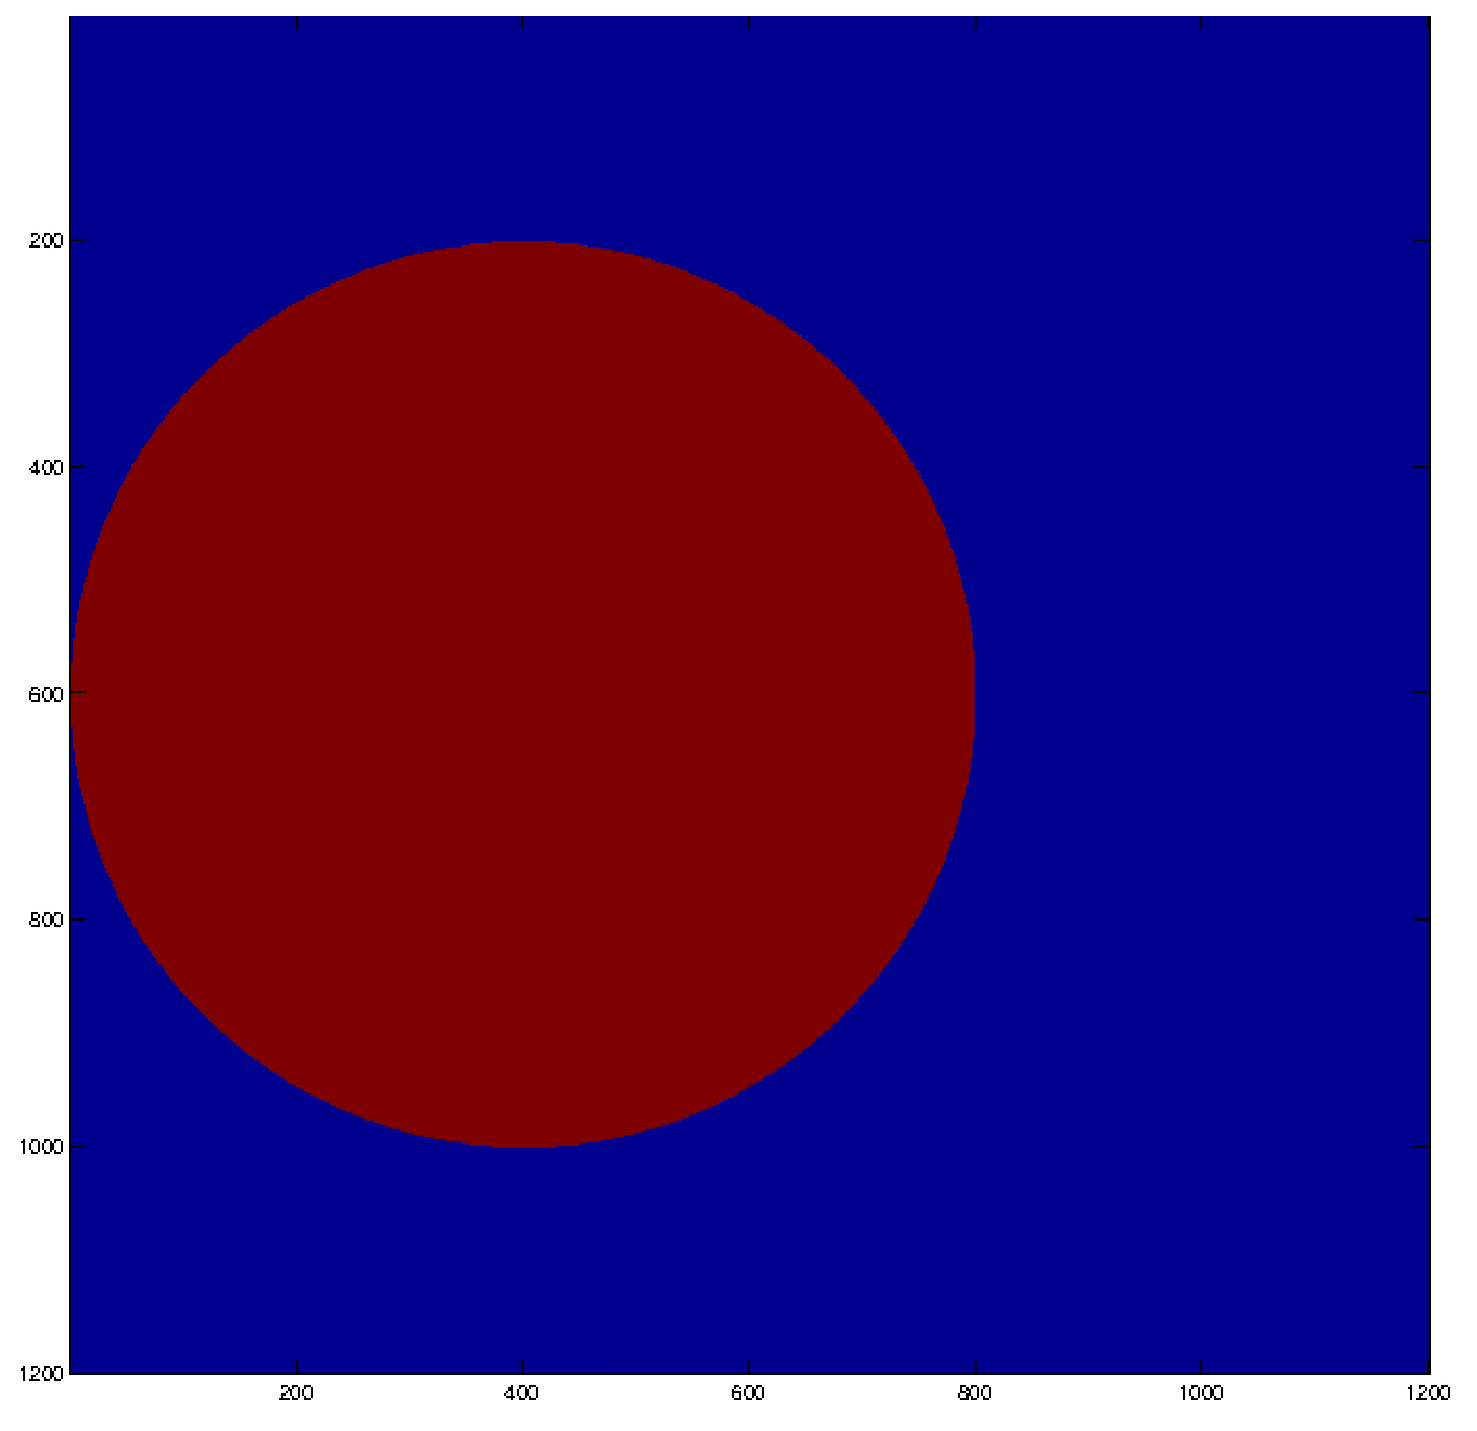
\includegraphics[width=\textwidth]{EPSFiles/Mandelbrot_Power_0}
                \caption{$d = 0$}
        \end{subfigure}
        \begin{subfigure}[b]{0.18\textwidth}
                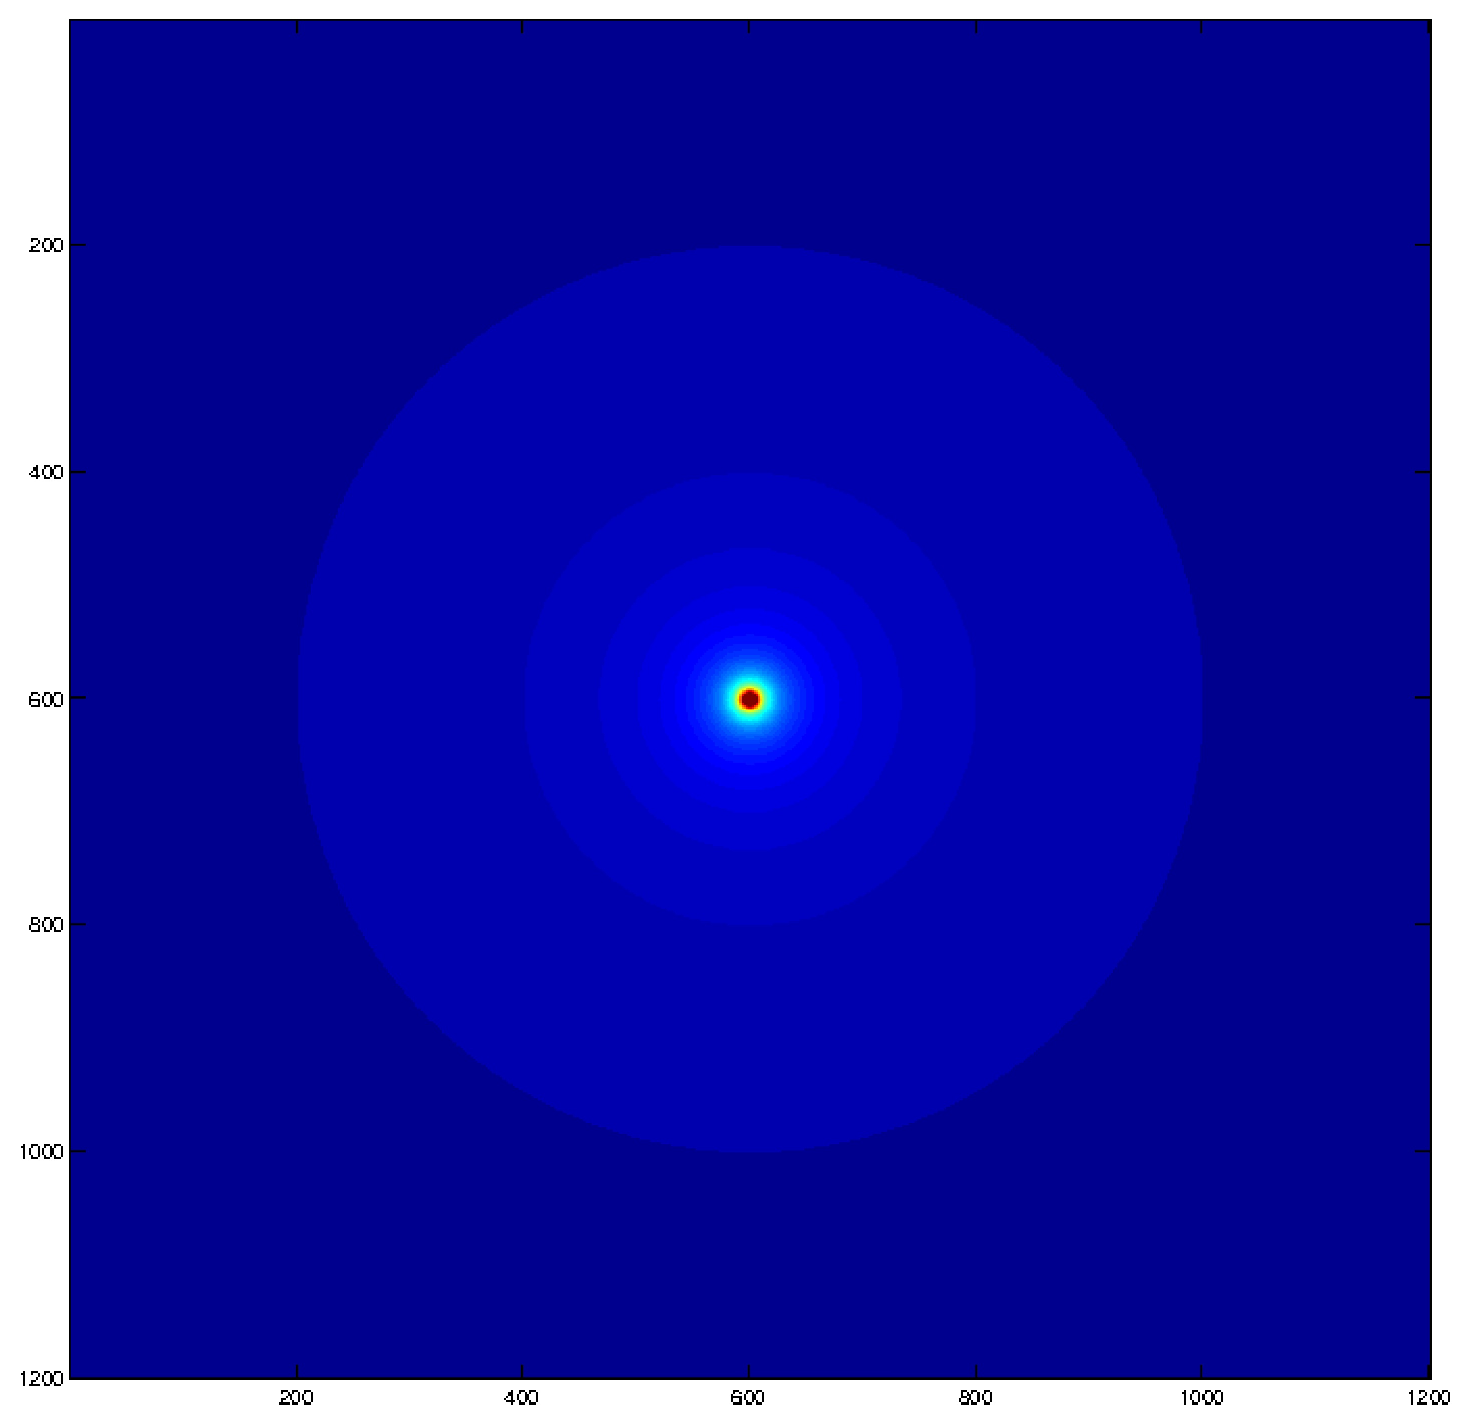
\includegraphics[width=\textwidth]{EPSFiles/Mandelbrot_Power_1}
                \caption{$d = 1$}
        \end{subfigure}
        \begin{subfigure}[b]{0.18\textwidth}
                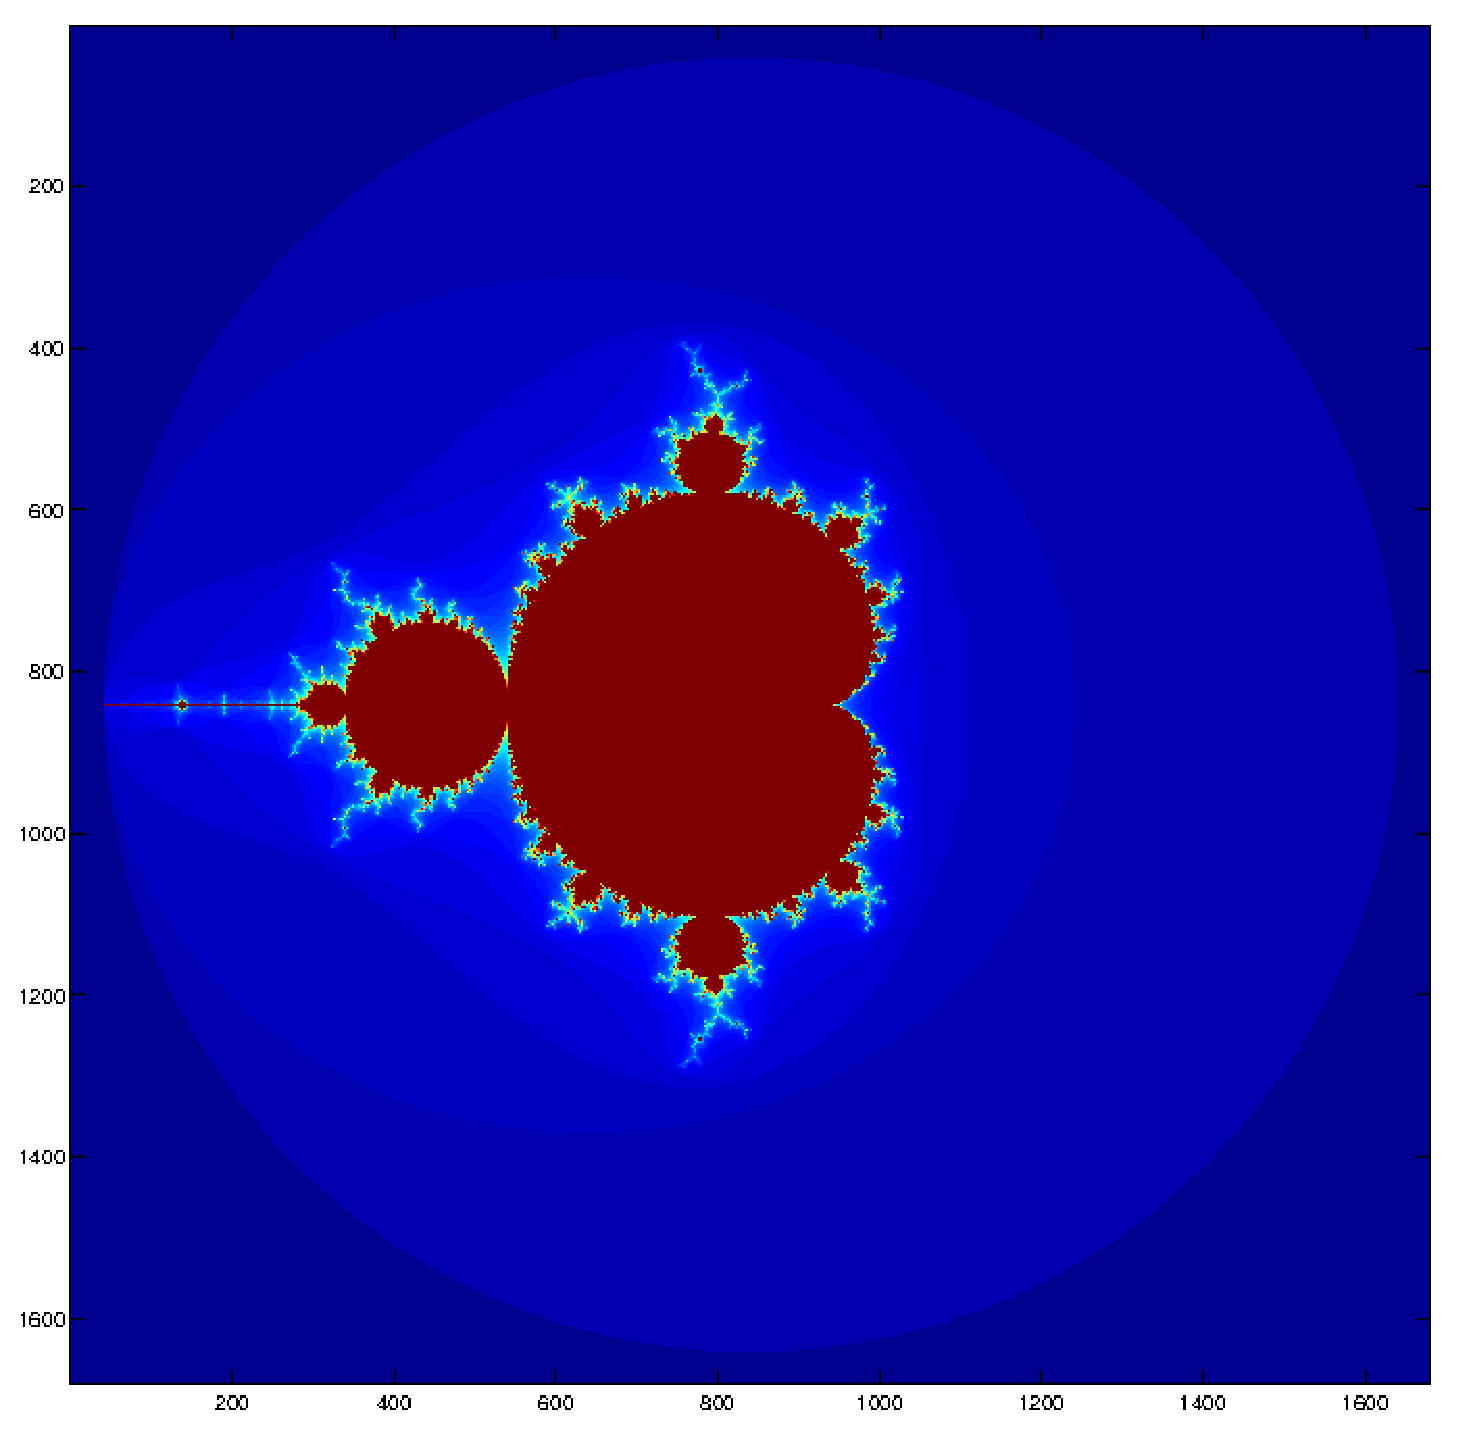
\includegraphics[width=\textwidth]{EPSFiles/Mandelbrot_Power_2}
                \caption{$d = 2$}
        \end{subfigure}        
        \begin{subfigure}[b]{0.18\textwidth}
                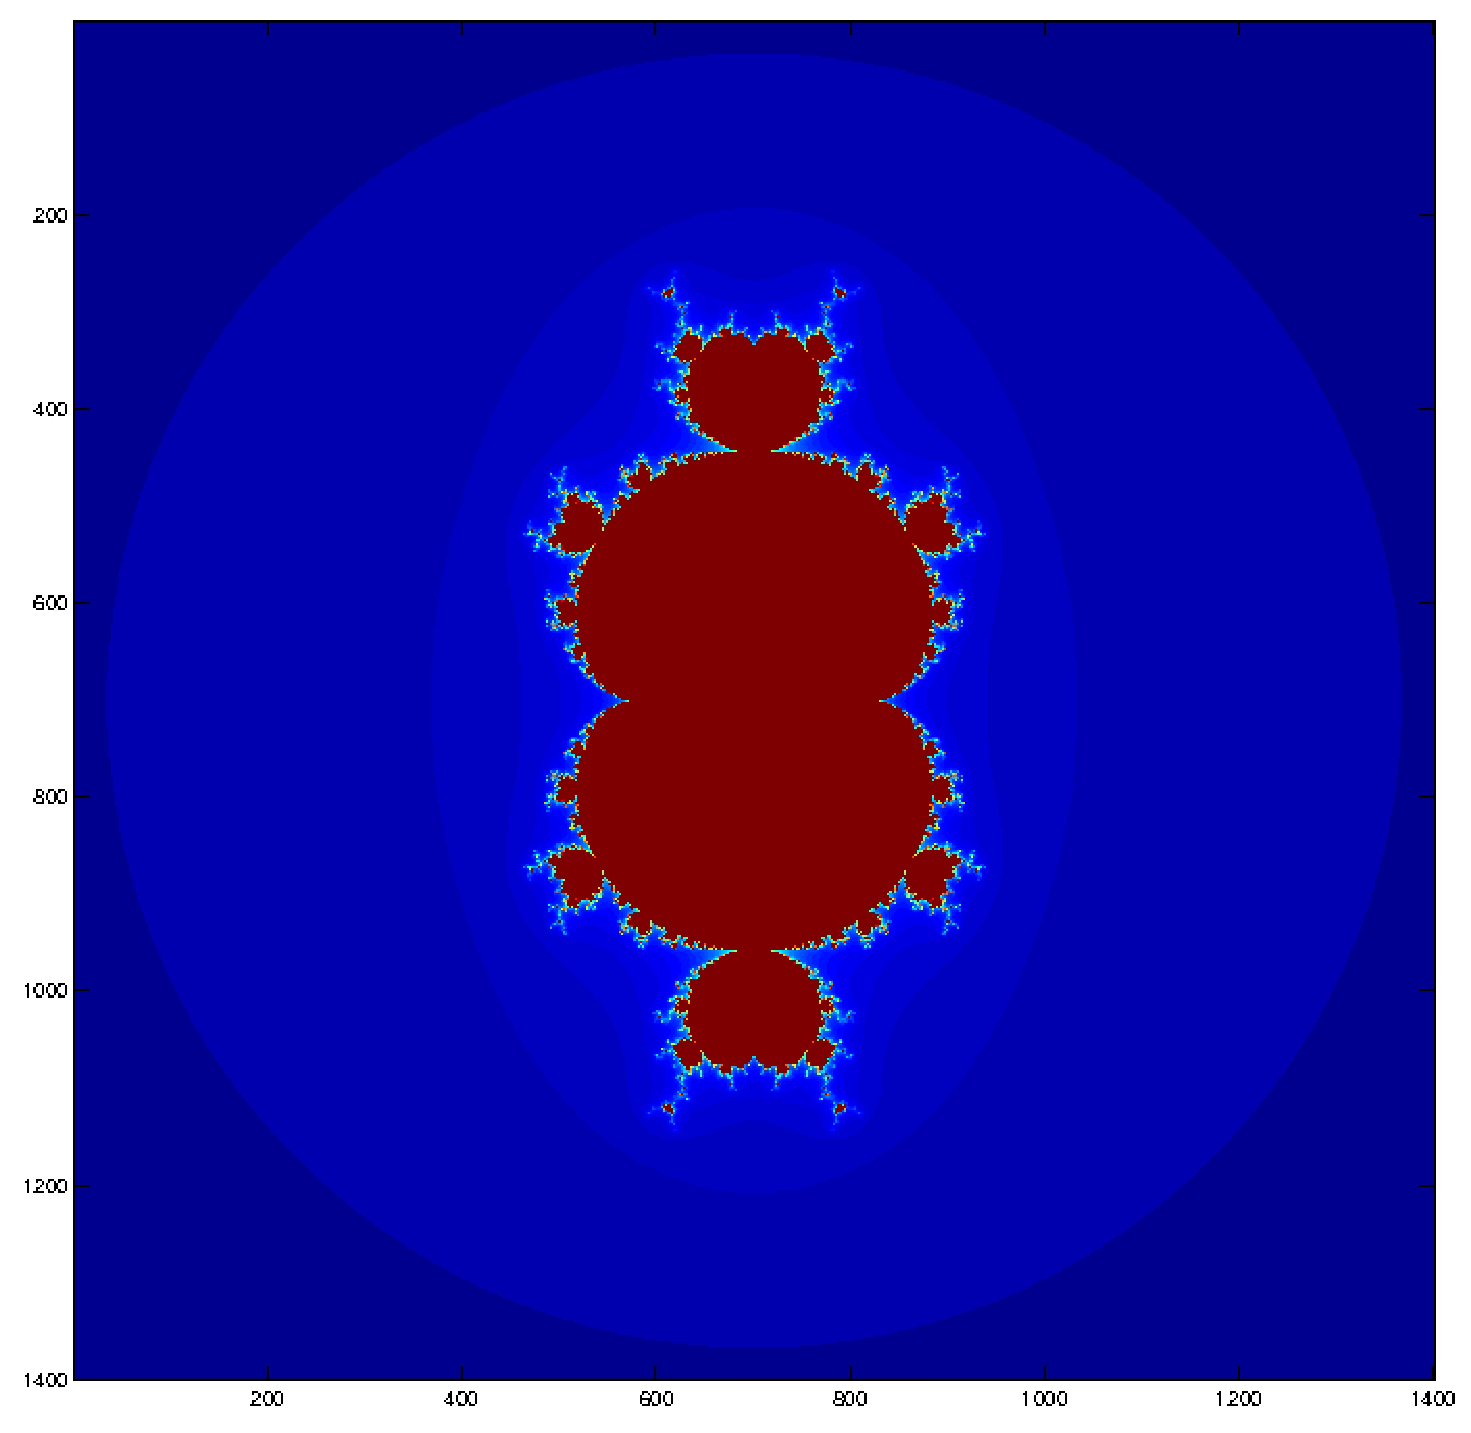
\includegraphics[width=\textwidth]{EPSFiles/Mandelbrot_Power_3}
                \caption{$d = 3$}
        \end{subfigure}
        \begin{subfigure}[b]{0.18\textwidth}
                \includegraphics[width=\textwidth]{EPSFiles/Mandelbrot_Power_4}
                \caption{$d = 4$}
        \end{subfigure}  
        \begin{subfigure}[b]{0.18\textwidth}
                \includegraphics[width=\textwidth]{EPSFiles/Mandelbrot_Power_5}
                \caption{$d = 5$}
        \end{subfigure}  
        \begin{subfigure}[b]{0.18\textwidth}
                \includegraphics[width=\textwidth]{EPSFiles/Mandelbrot_Power_6}
                \caption{$d = 6$}
        \end{subfigure} 
        \begin{subfigure}[b]{0.18\textwidth}
                \includegraphics[width=\textwidth]{EPSFiles/Mandelbrot_Power_7}
                \caption{$d = 7$}
        \end{subfigure} 
        \caption{Changing power of z for Mandelbrot set.}
\end{figure}

Special cases when $d = 0$ show that the image produced is actually a circle of diameter 1, this is due
 to the fact that $|z| \textrm{ for the constant expression } z = 1 + c$ is always in the set when $|c|
  \leq 1$ as this would ensure $|z| \leq 2$. On another note when $d = 1$ we see a small region in the
   center of the image showing some c values to be inside the Mandelbrot set, theoretically, there
    should not be any values of c in the set as the equation produced by this iterative process is $z =
     1 + c + c + c + c + ...$ which is unbounded for any value of c. To show this unbounded nature at
      $d = 1$ accurately we would have to perform an infinite amount of iterations as $z > 2$ at some
       point due to it's unbounded nature in this case. The rest of the images above follow the pattern
        of symmetry as described previously.

%Conversely negative powers of the \emph{MultiBrot Set} %how a $(1-d) \textrm{- fold rotational
% symmentry}$ with most c values lying in the set at %points around the origin, creating interesting
%  fractal designs in the center. There are also images %of fractional powers above.

%\section{References 'cause I don't know where else to put these yet REMEMBER TO CHANGE THIS TO MAKE IT ALL FANCY AND STUFF}

% arxiv.org/pdf/0910.1560.pdf I don't even know what to use this for, it just sounded good

% \emph{YOUTUBE VIDEO OF FRACTAL} PUT THIS IN PRESENTATION OR KIRAN WILL CRY :'(

%\subsection{Helpful links}

%http://www.win.tue.nl/~setalle/introduction.html

%http://www.mathworks.com/matlabcentral/answers/96084-how-do-i-include-a-matlab-figure-in-a-latex-document

\begin{thebibliography}{20}

\bibitem{Chaos in Dictionary}
  Oxford Dictionary, 
  "Defintion of chaos in the dictionary",
  http://www.oxforddictionaries.com/definition/english/chaos.
  
\bibitem{Pierre Verhulst Biography}
  J. J. O'Connor and E. F. Robertson, 
  "Verhulst biography", 
  2014, 
  http://www-history.mcs.st-andrews.ac.uk/Biographies/Verhulst.html.
  
\bibitem{Information on Veruhlst and Verhulst/Logistic Maps}
  N. Baca\"er, 
  \emph{"A Short History of Mathematical Population Dynamics"}, 
  Springer-Verlag London Limited, 
  2011, 
  https://masalladelaespecie.files.wordpress.com/2015/01/verhlogeq.pdf.
  
%KIRAN THIS IS THE GOOGLE BOOK IF YOU WANNA REFERENCE IT
\bibitem{Verhulst Map Period Doubling Information}
  Keith J. Devlin, 
  \emph{Mathematics: The New Golden Age}, 
  Pages 100 - 102, 
  Columbia University Press, 
  1999.
  
\bibitem{Butterfly Effect}
  James Gleick, 
  \emph{Chaos}
  Pages 16 - 18, 
  Vintage Books London, 
  1998.

\bibitem{Julia definition}
Weisstein, Eric W,
"Julia set",
 2015,
 http://mathworld.wolfram.com/JuliaSet.html

\bibitem{compactness}
  The editors of Encyclopaedia Britannica,
  "Compactness",
  2015,
 http://www.britannica.com/EBchecked/topic/129532/compactness

\bibitem{compact proof}
 Dalibor Praˇz´ak,
 "The Mandelbrot Set",
 2000,
 http://www.karlin.mff.cuni.cz/~prazak/doc/mandel.pdf

\bibitem{Fractal Properties}
  Edyta Patrzalek, 
  \emph{Fractals: Useful Beauty}, 
  "Properties of a fractal", 
  2008, 
  http://www.fractal.org/Bewustzijns-Besturings-Model/Fractals-Useful-Beauty.htm.

\bibitem{Bifurcation in Mandelbrot Set 1}
  Wikimedia user Hoehue,
  "Mandelbrot Period Doubling",
  2005, 
  \url{http://commons.wikimedia.org/wiki/File:Mandelbrot_Set_%E2%80%93_Periodicities_coloured.png}.
  
\bibitem{Bifurcation in Mandelbrot Set 2}
  Georg-Johann Lay,
  "Image showing Bifurcation in the Mandelbrot set with Verhulst",
  2008, 
  http://commons.wikimedia.org/wiki/File:Verhulst-Mandelbrot-Bifurcation.jpg
  
\bibitem{Understanding Julia Sets}
  Karl Sims,
  "Understanding Julia Sets", 
  http://www.karlsims.com/julia.html
  
\bibitem{Mandelbrot Set Matlab}
  Cleve Moler,
  "Matlab Mandelbrot Examples",
  2011, 
  http://uk.mathworks.com/moler/exm/chapters/mandelbrot.pdf

\bibitem{Jay Hill}
 Dr Mark Haskins,
 "$\pi$ in the Mandelbrot Set",
 2001,
 \url{http://www.math.jhu.edu/~mhaskin/teaching/ug_research/mandelbrot.pdf}

\bibitem{Boll proof}
 Aaron Klebanoff,
 "$\pi$ in the Mandelbrot set",
 2001,
 http://www.worldscientific.com/doi/pdfplus/10.1142/S0218348X01000828

\bibitem{Proof for $|z|<= 2$}
  Robert P. Munafo,
  "Proof for why $|z|<= 2$ in the iterative process ", 1997, 
  http://mrob.com/pub/muency/escaperadius.html
>>>>>>> 20e35ade04b166ba06e6a720ad39b286e5b0db3f
%TAKE THESE OUT - THEY ARE JUST EXAMPLES

%\bibitem{bookExample}
%  Author(s),
%  \emph{Book name}.
%  Publisher,
%  Edition if any,
% Year FULL STOP.
  
%\bibitem{websiteExample}
%  Name of a person - just find one :p,
%  "Description",
%  year, 
%  URL.

\end{thebibliography}

\end{document}